\label{Beispiele}
\chapter{Beispielsitzung}

	Auf den nächsten Seiten sind einige Bildschirmabzüge des CoachingBots zu sehen. Zunächst wird durch eine Sitzung aus Sicht des Nutzers geführt, bevor die Ansichtdes Coaches gezeigt wird.\\ 
	\\
	Der Nutzer startet den Bot via dem Klick auf einen Link\footnote{\url{https://t.me/thecoachingbot?start=start}}, den er auf einer Website findet oder der ihm zugesandt wird.

	% PAGE 01
	\begin{figure}
		\centering
		\begin{minipage}{.48\linewidth}
		  \centering
		  \subcaptionbox{Einstieg via URL}
			{
\includegraphics[width=\linewidth,height=150pt,keepaspectratio]{images/Screenshots/link.png}}
	  
		  \subcaptionbox{Start des CoachingBots}
			{
\includegraphics[width=\linewidth,height=300pt,keepaspectratio]{images/Screenshots/start.PNG}}
	  
		  \caption{Einstieg und Start}
		\end{minipage}\quad
		\begin{minipage}{.48\linewidth}
		  \centering
		  \subcaptionbox{Übergang zur Angabe der Biographie}
			{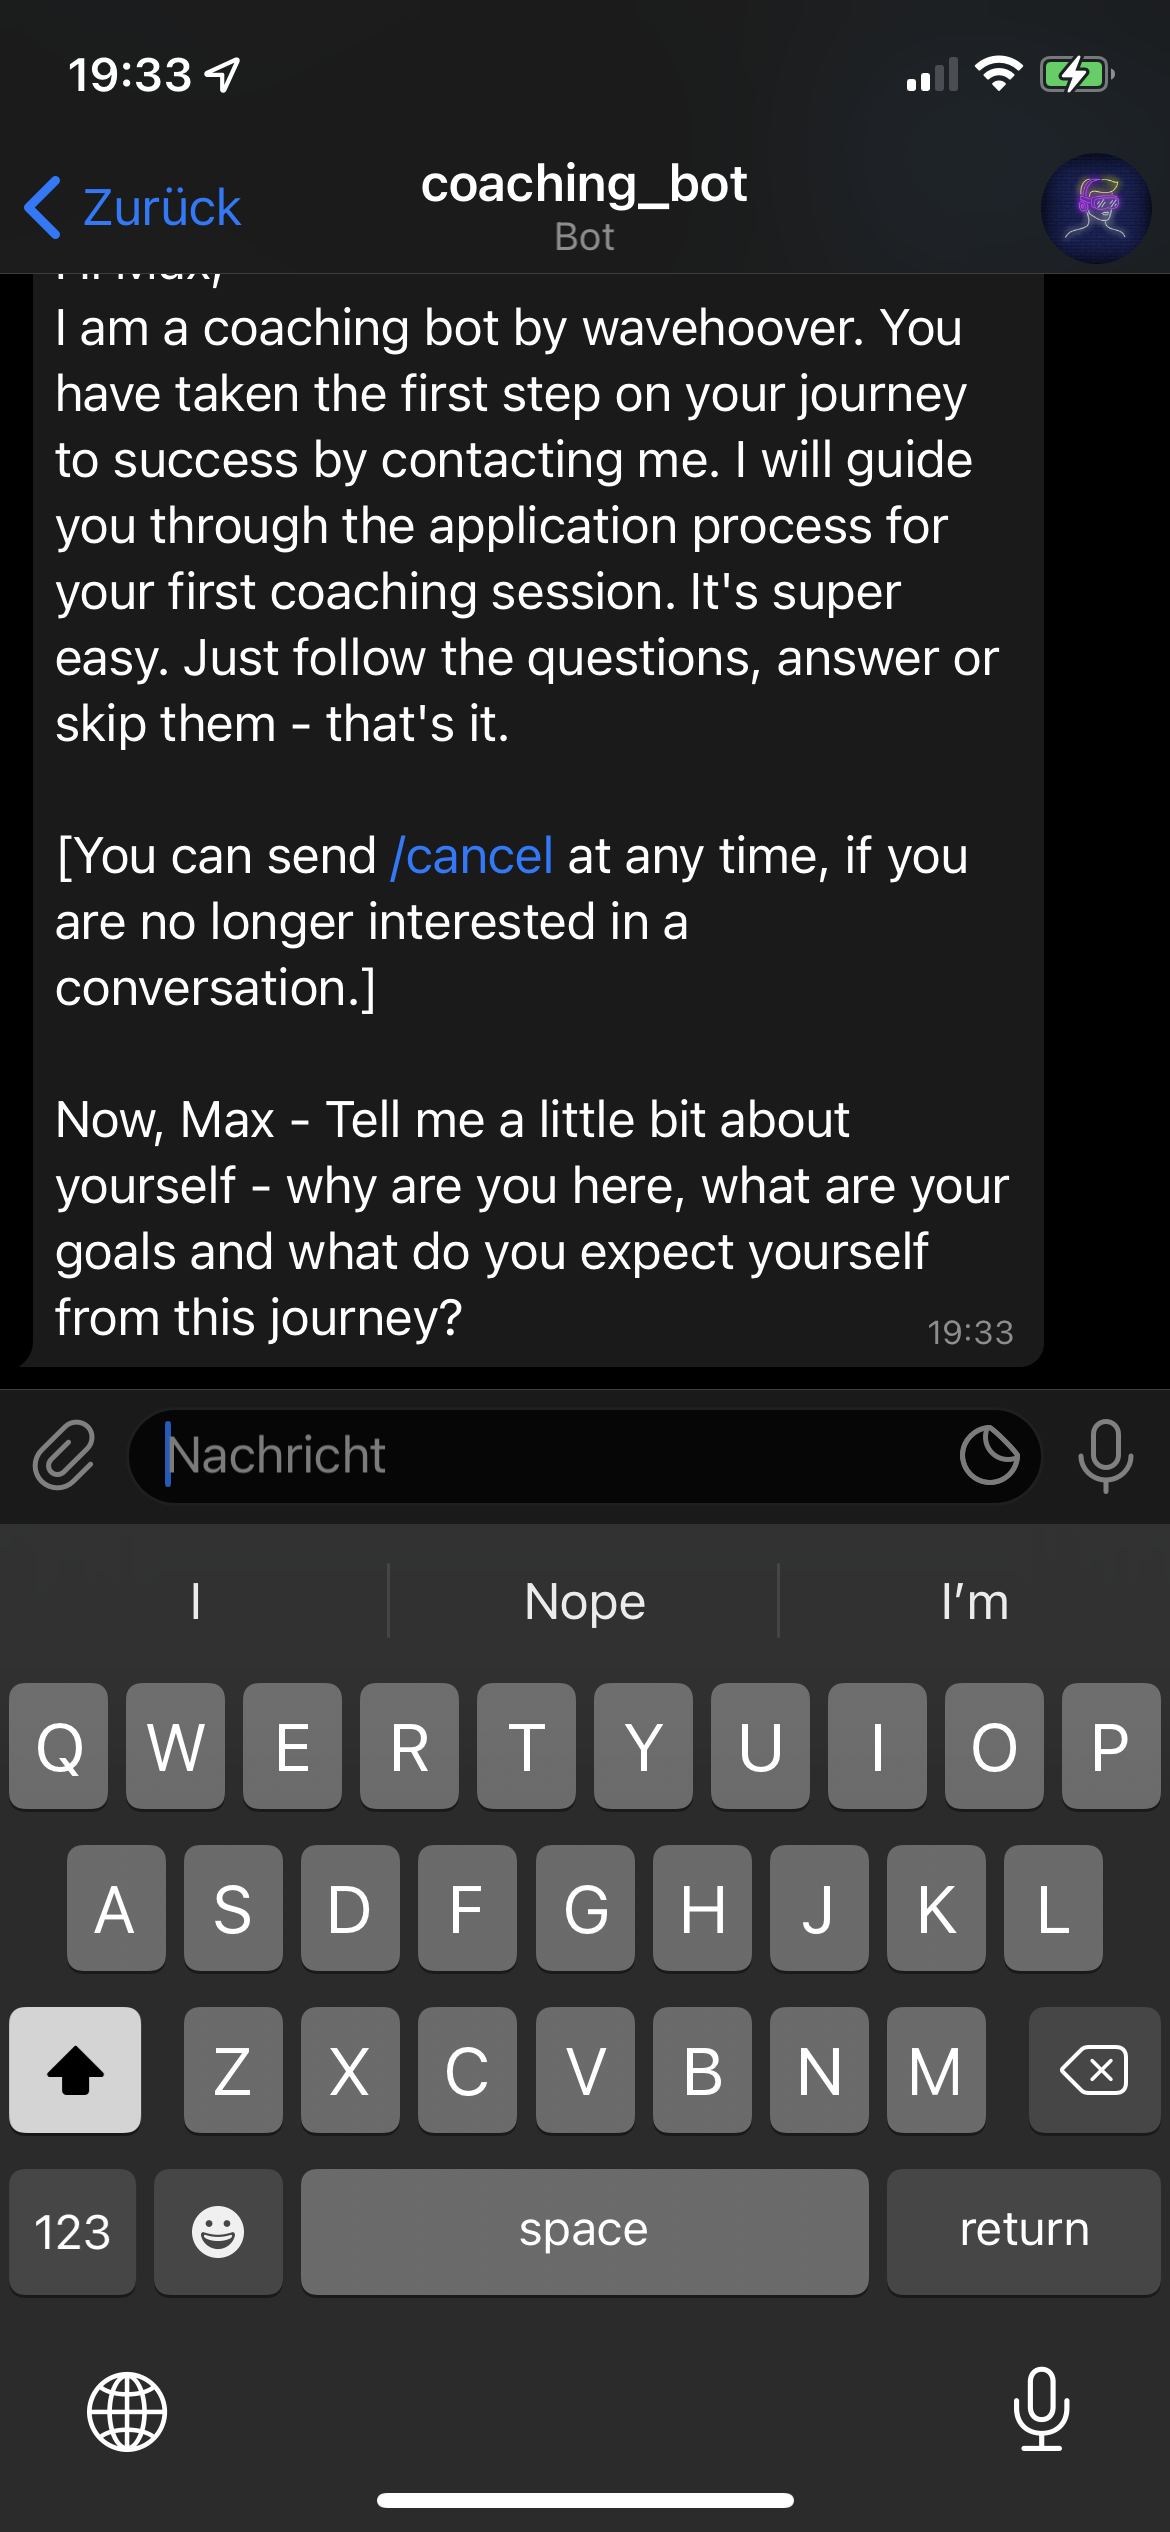
\includegraphics[width=\linewidth,height=300pt,keepaspectratio]{images/Screenshots/bio.PNG}}
	  
		  \subcaptionbox{Übergang zur Auswahl des Geschlechts}
			{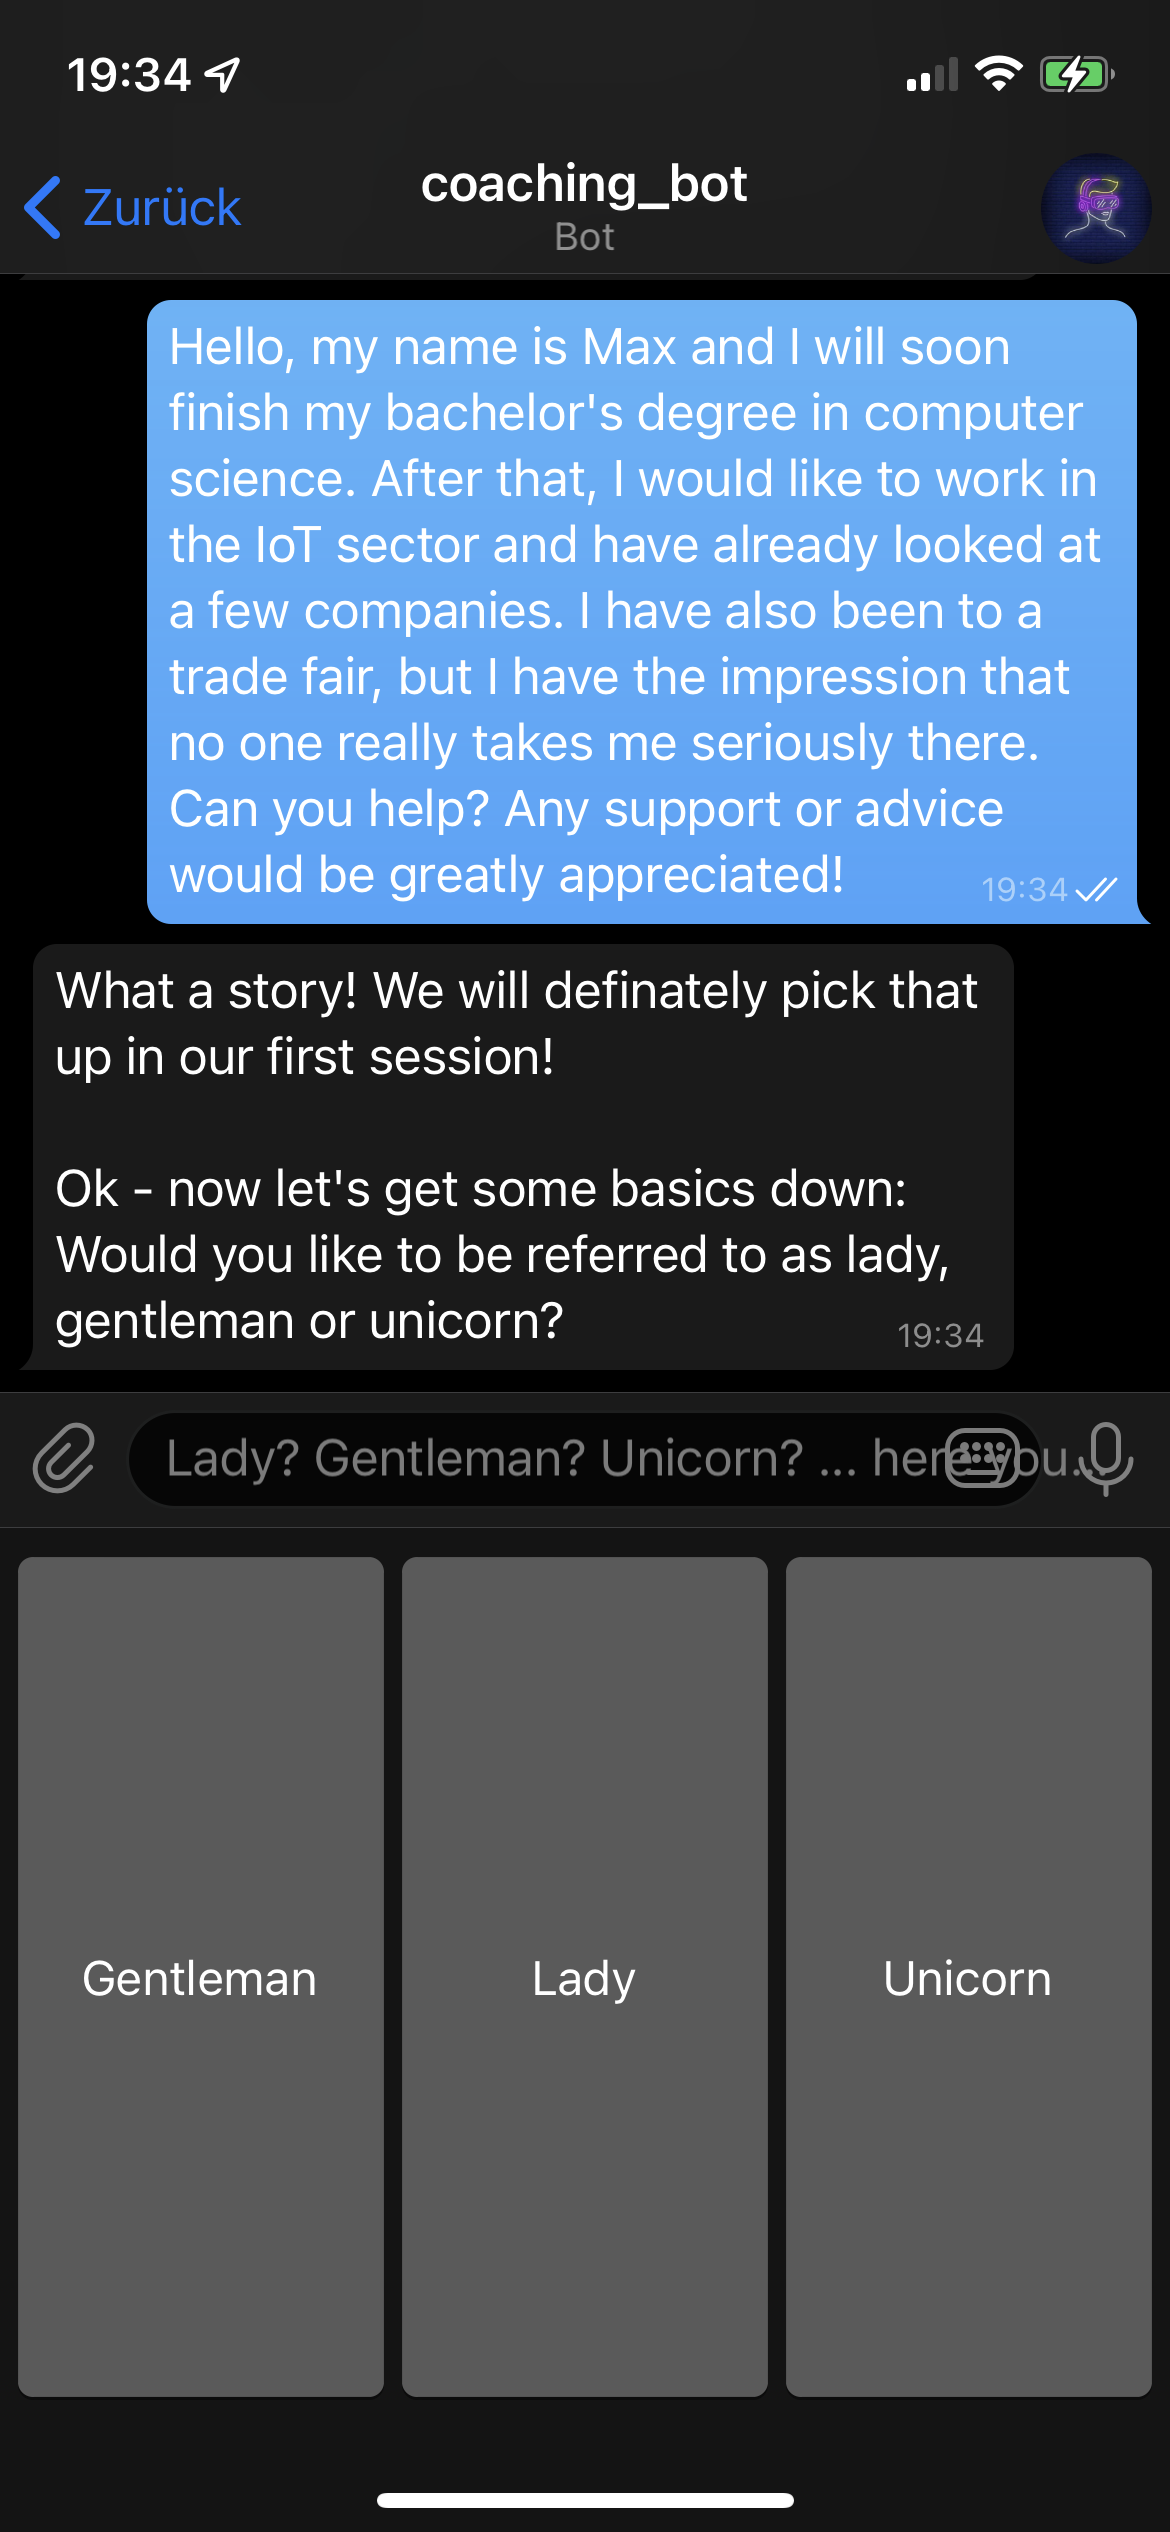
\includegraphics[width=\linewidth,height=300pt,keepaspectratio]{images/Screenshots/gender.PNG}}
	  
		  \caption{Erste Zustands-Übergänge}
		\end{minipage}
	\end{figure}


	% PAGE 02
	\begin{figure}
		\centering
		\begin{minipage}{.48\linewidth}
			\centering
			\subcaptionbox{Übergang zur Angabe des Geburtsdatums}
			{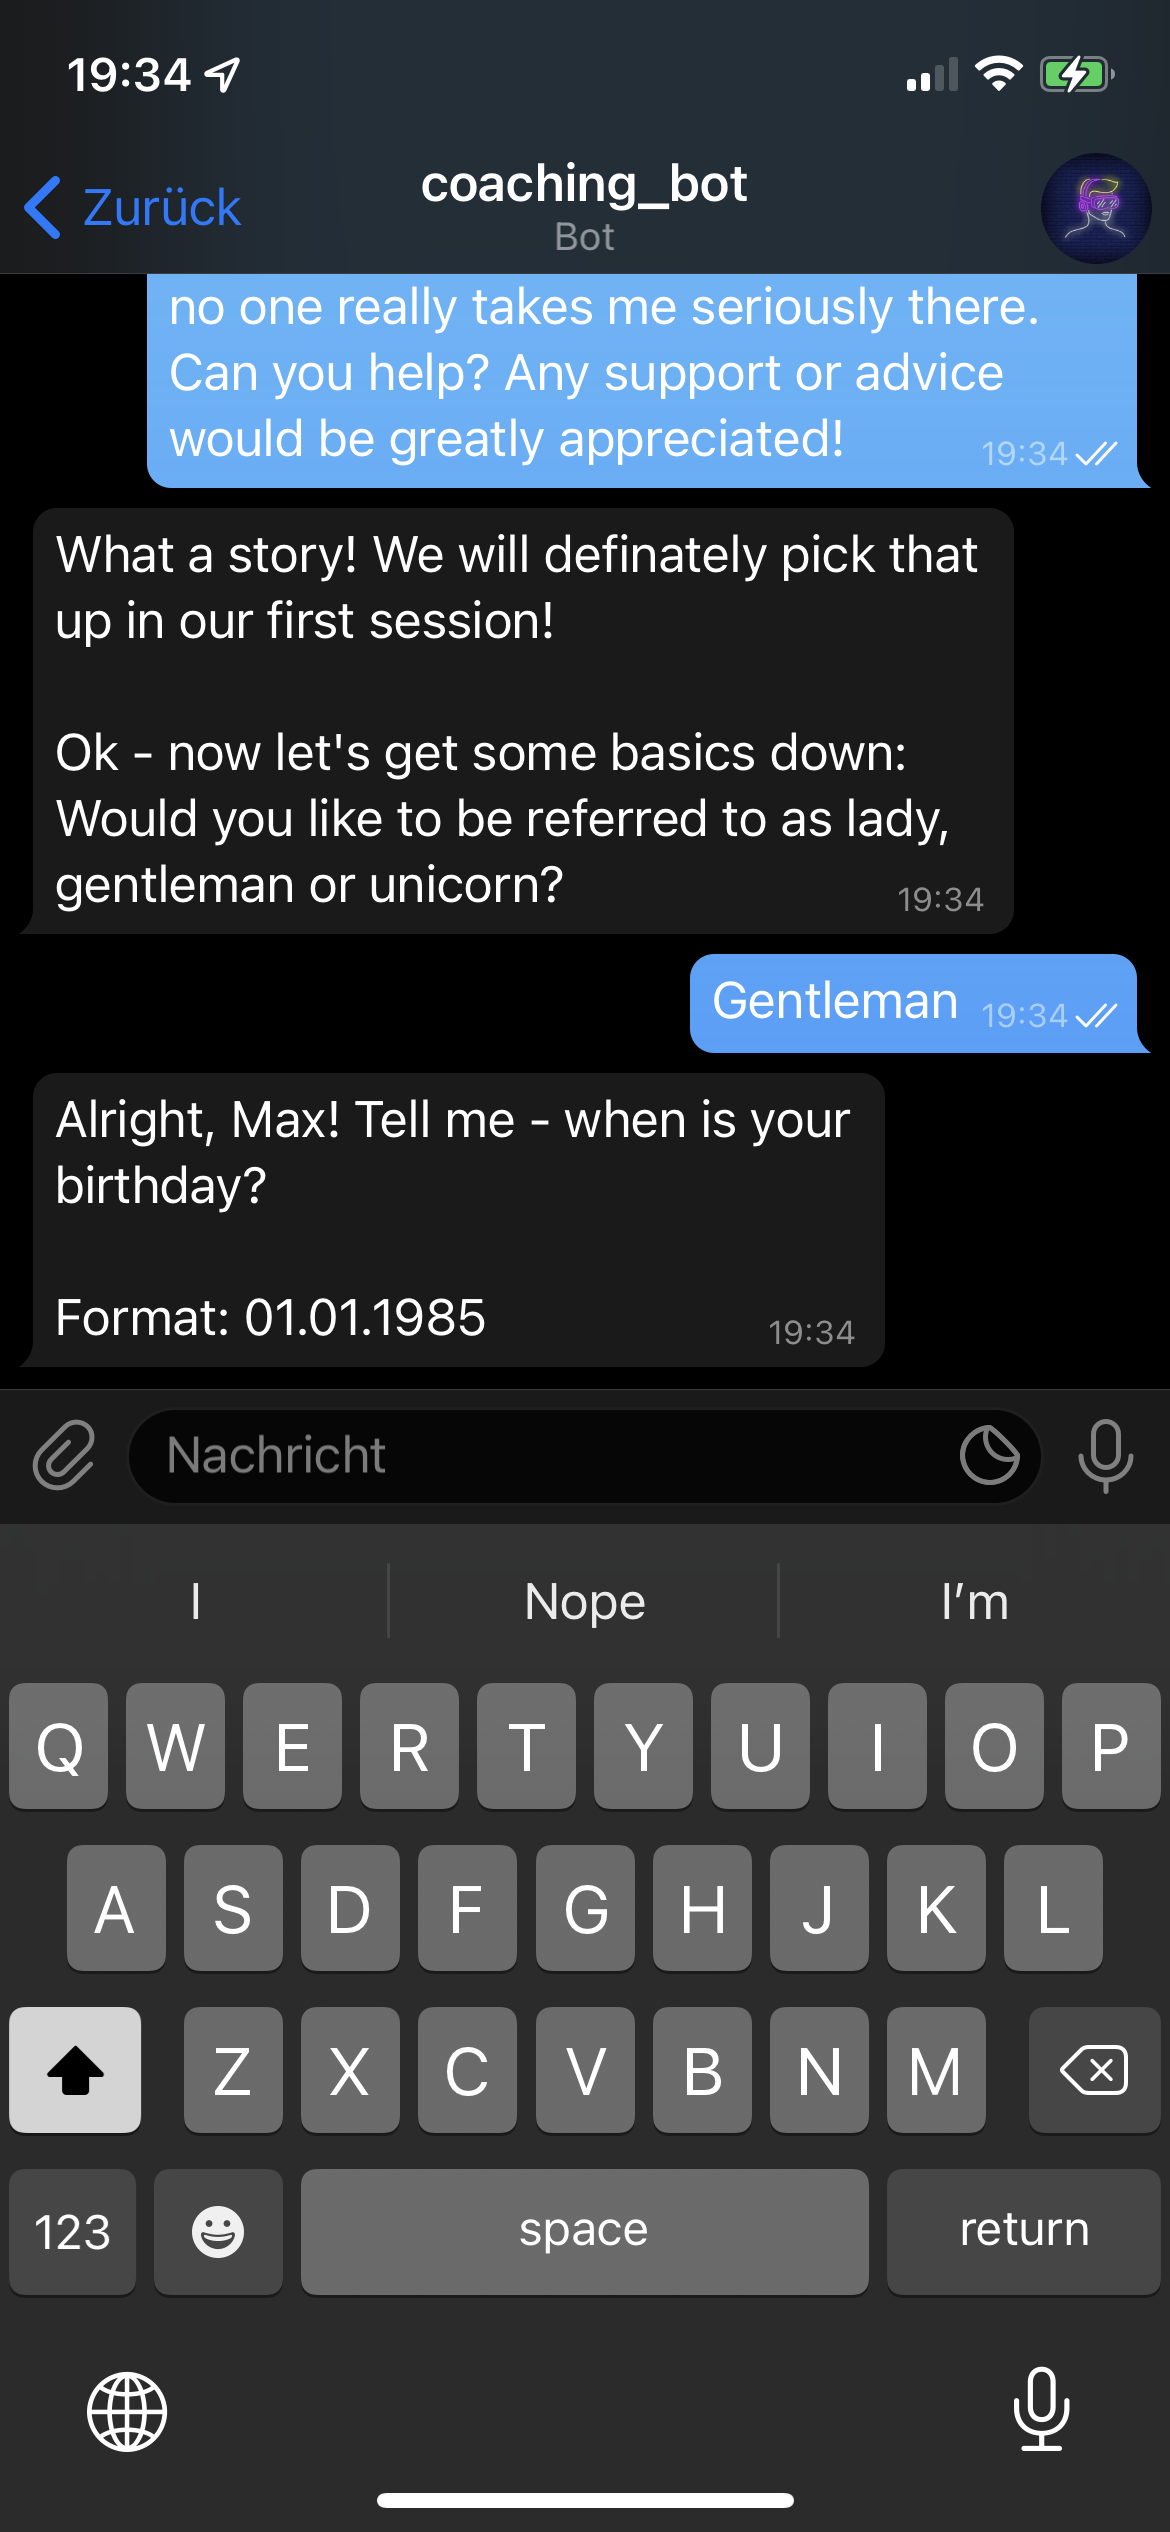
\includegraphics[width=\linewidth,height=300pt,keepaspectratio]{images/Screenshots/birthdate.PNG}}
		
			\subcaptionbox{Übergang zur Angabe der E-Mail-Adresse}
			{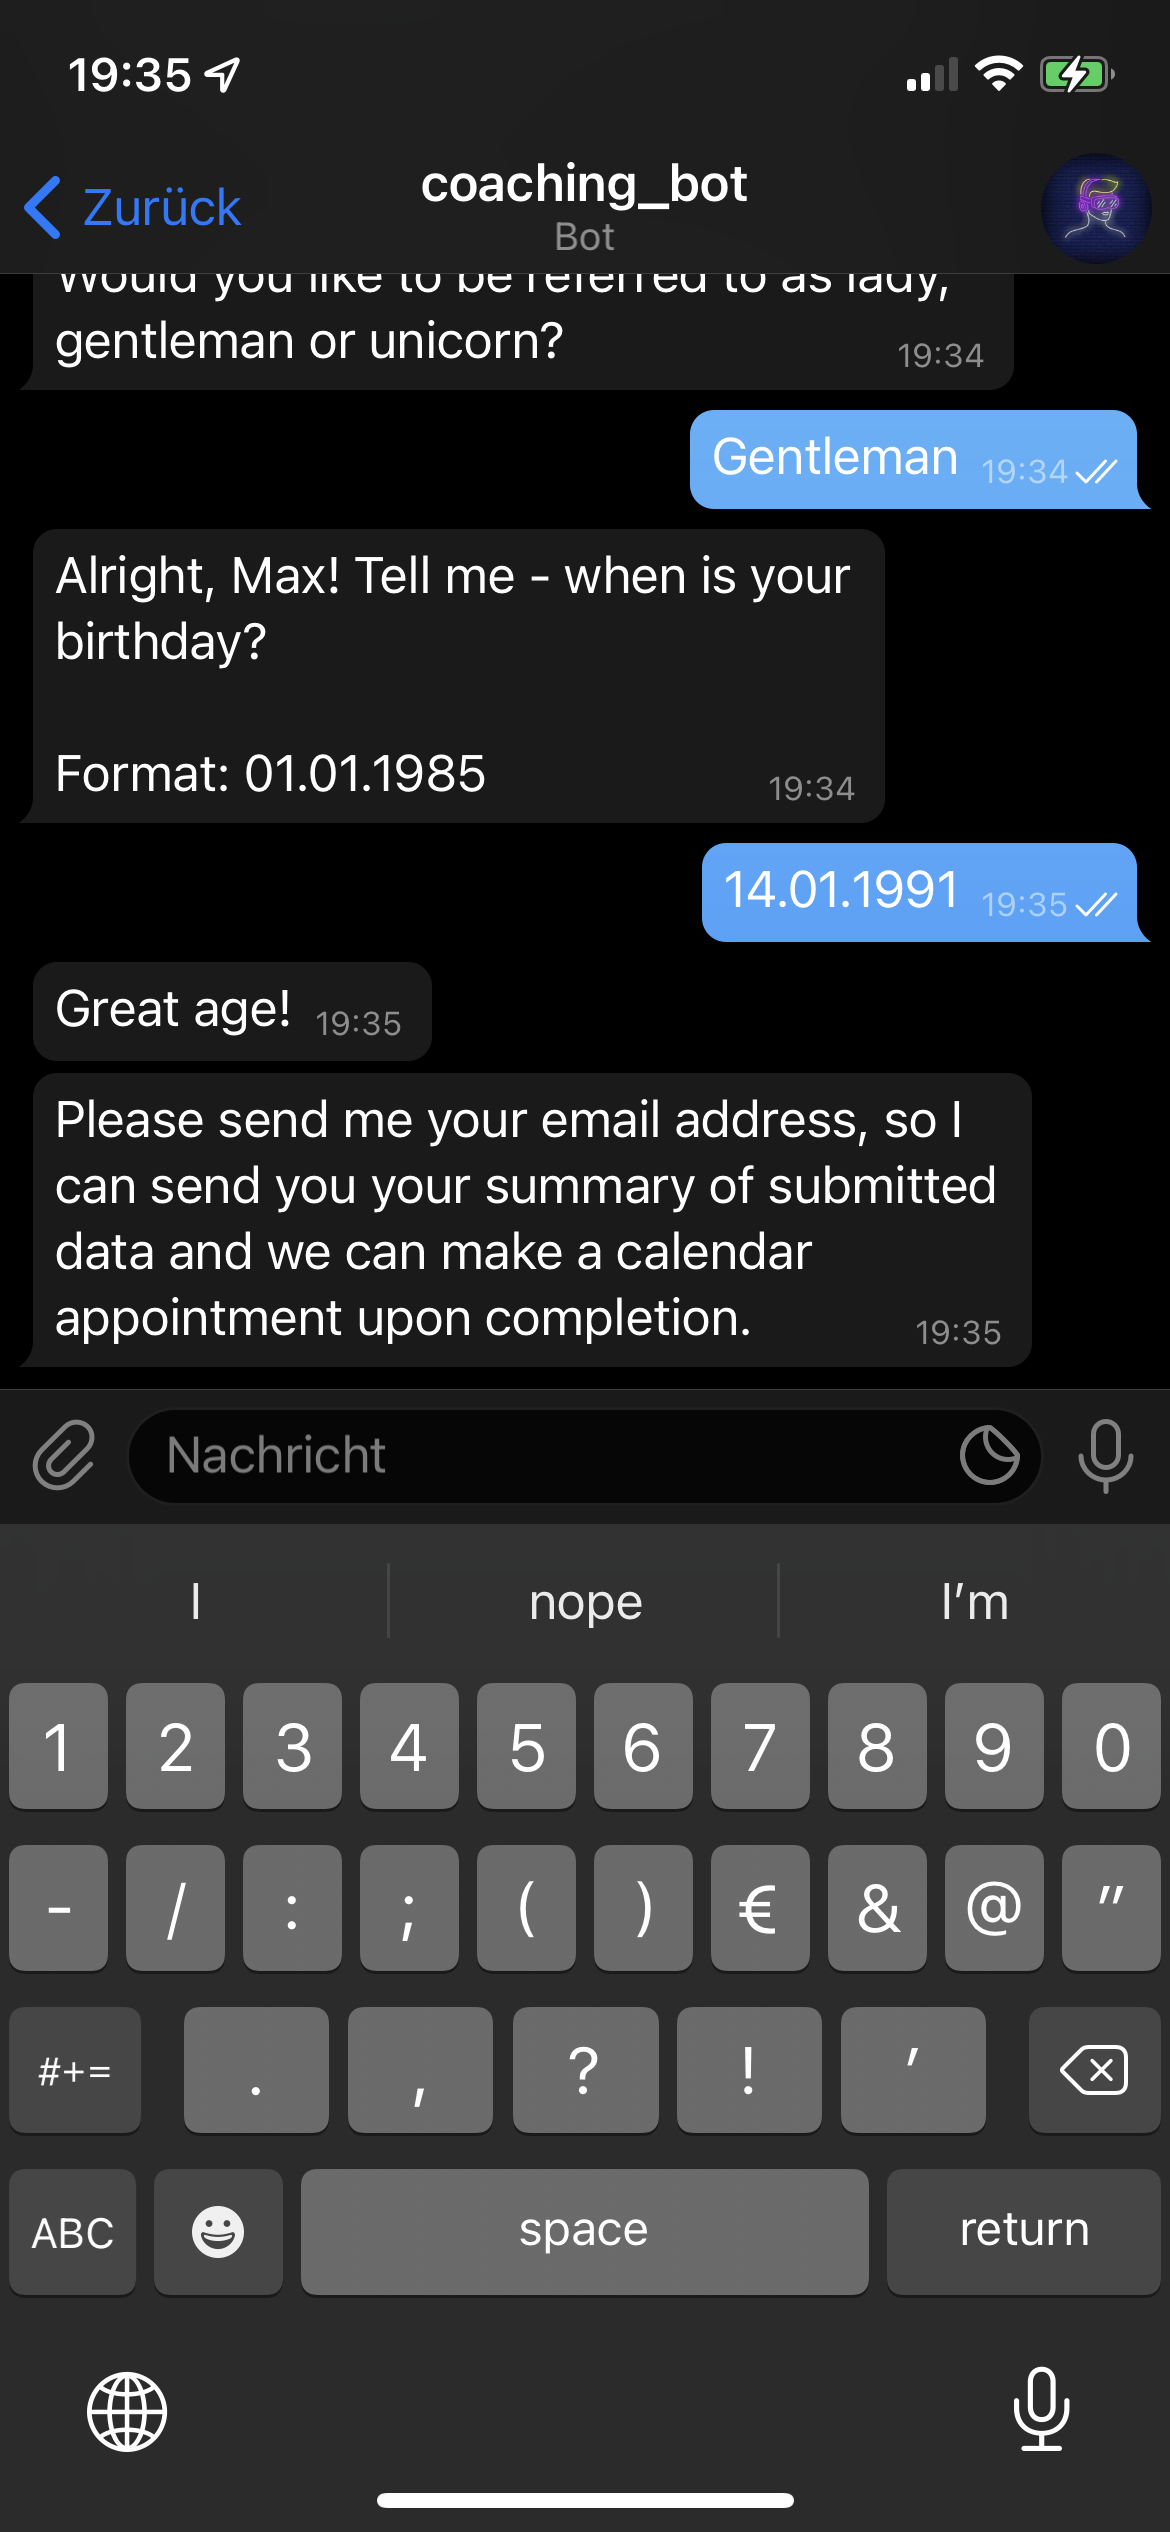
\includegraphics[width=\linewidth,height=300pt,keepaspectratio]{images/Screenshots/email.PNG}}
		
			\caption{Abfrage Geburtsdatum und E-Mail-Adresse}
		\end{minipage}\quad
		\begin{minipage}{.48\linewidth}
			\centering
			\subcaptionbox{Übergang zur Angabe der Telefonnummer}
			{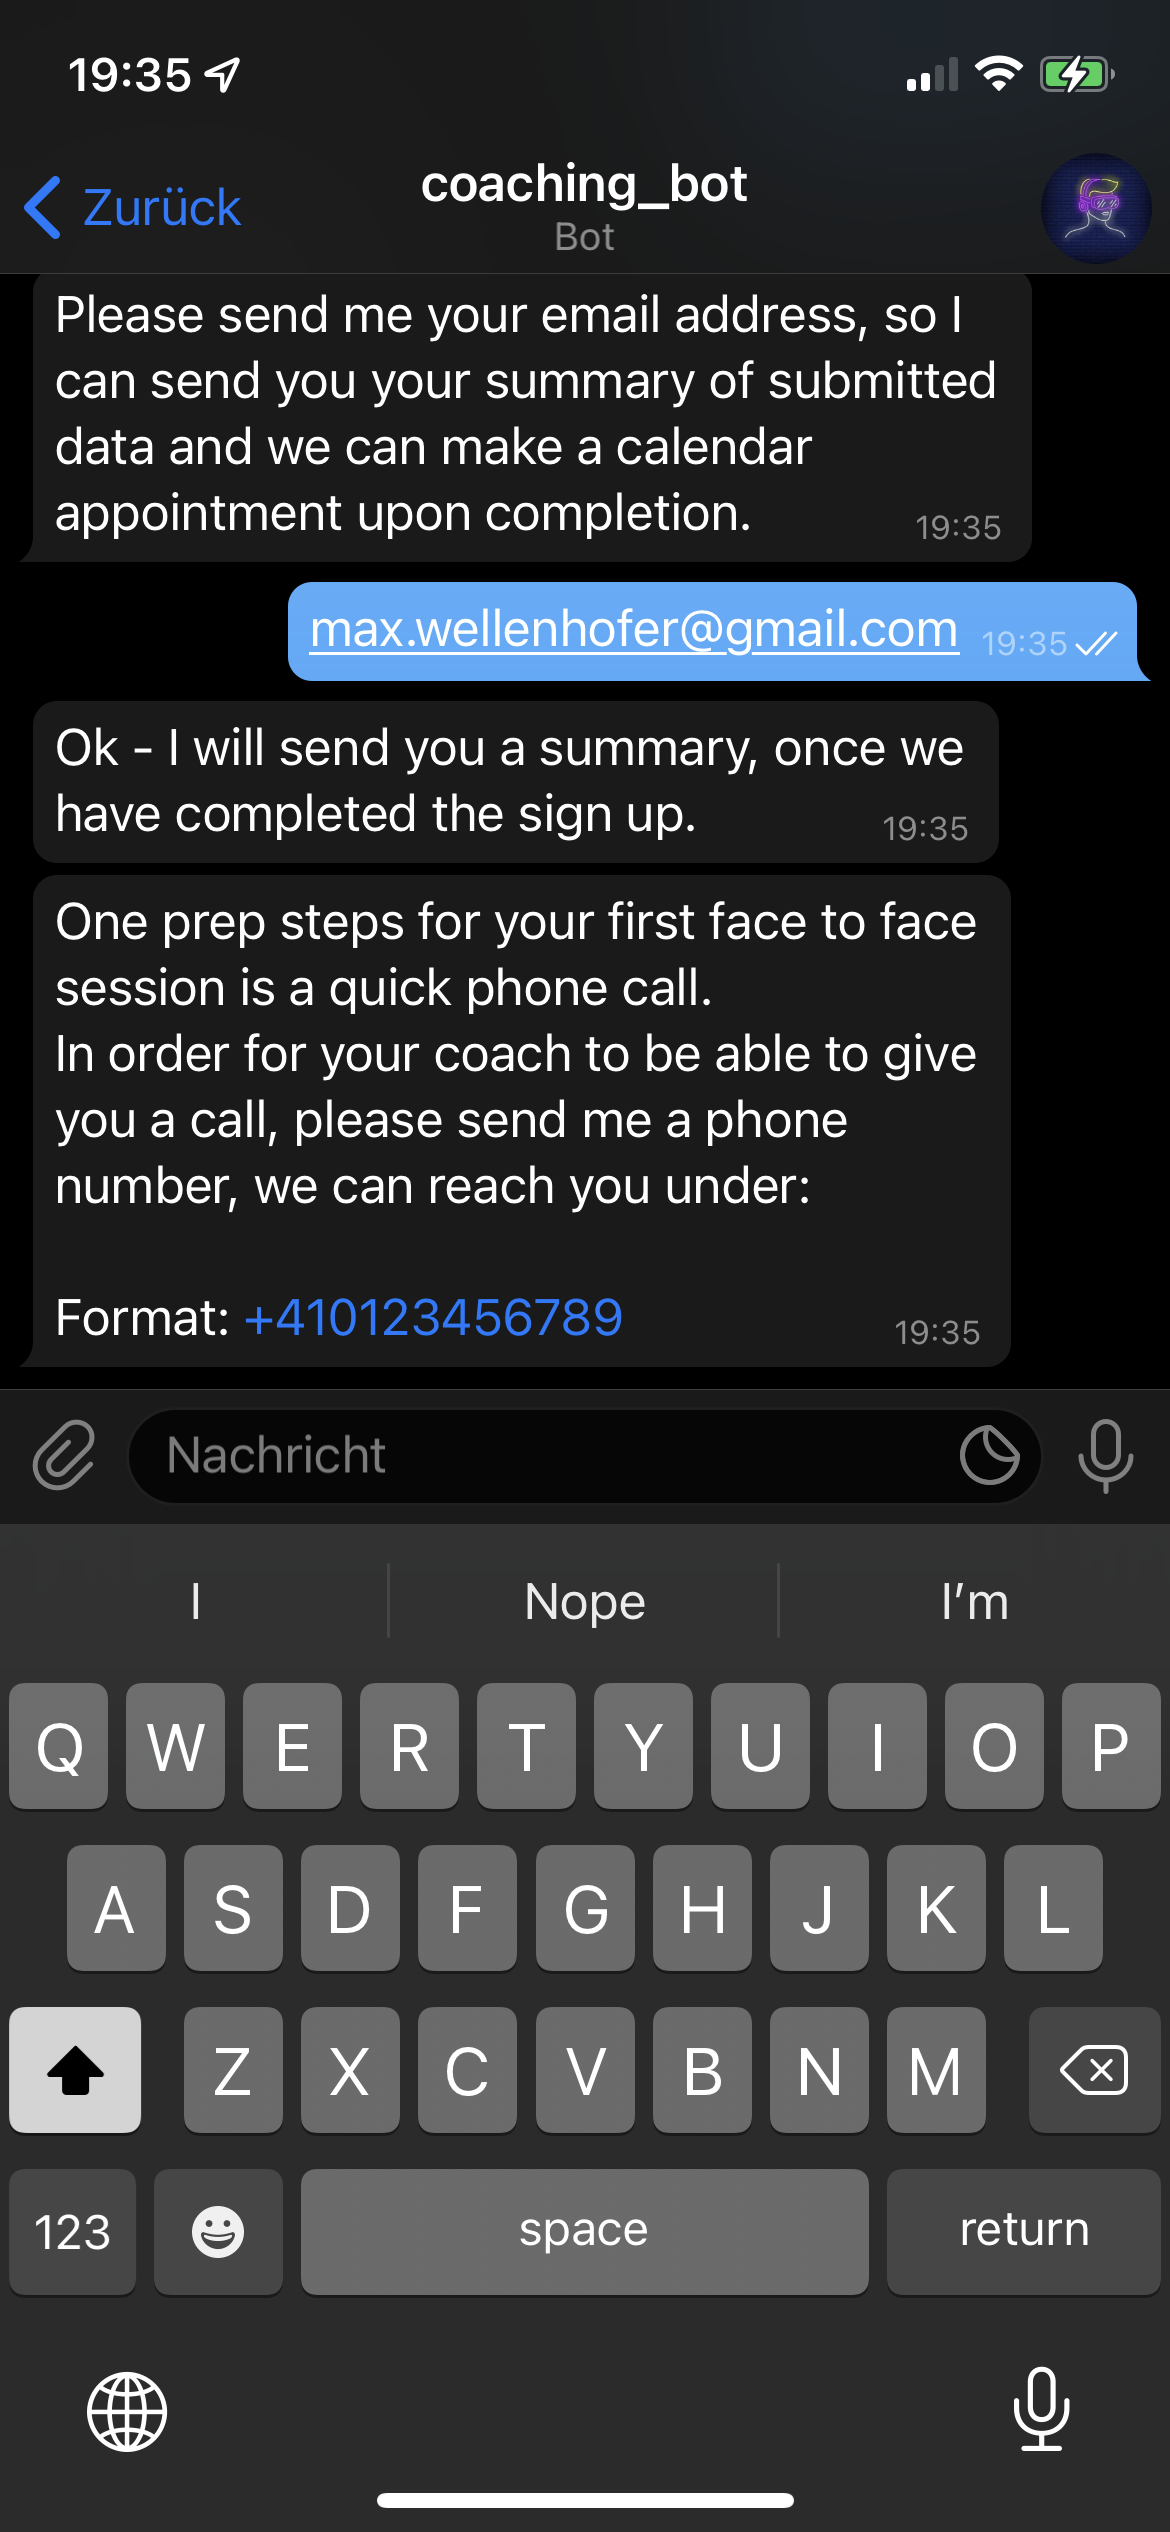
\includegraphics[width=\linewidth,height=300pt,keepaspectratio]{images/Screenshots/telephone.PNG}}
		
			\subcaptionbox{Übergang zur Angabe des Standorts}
			{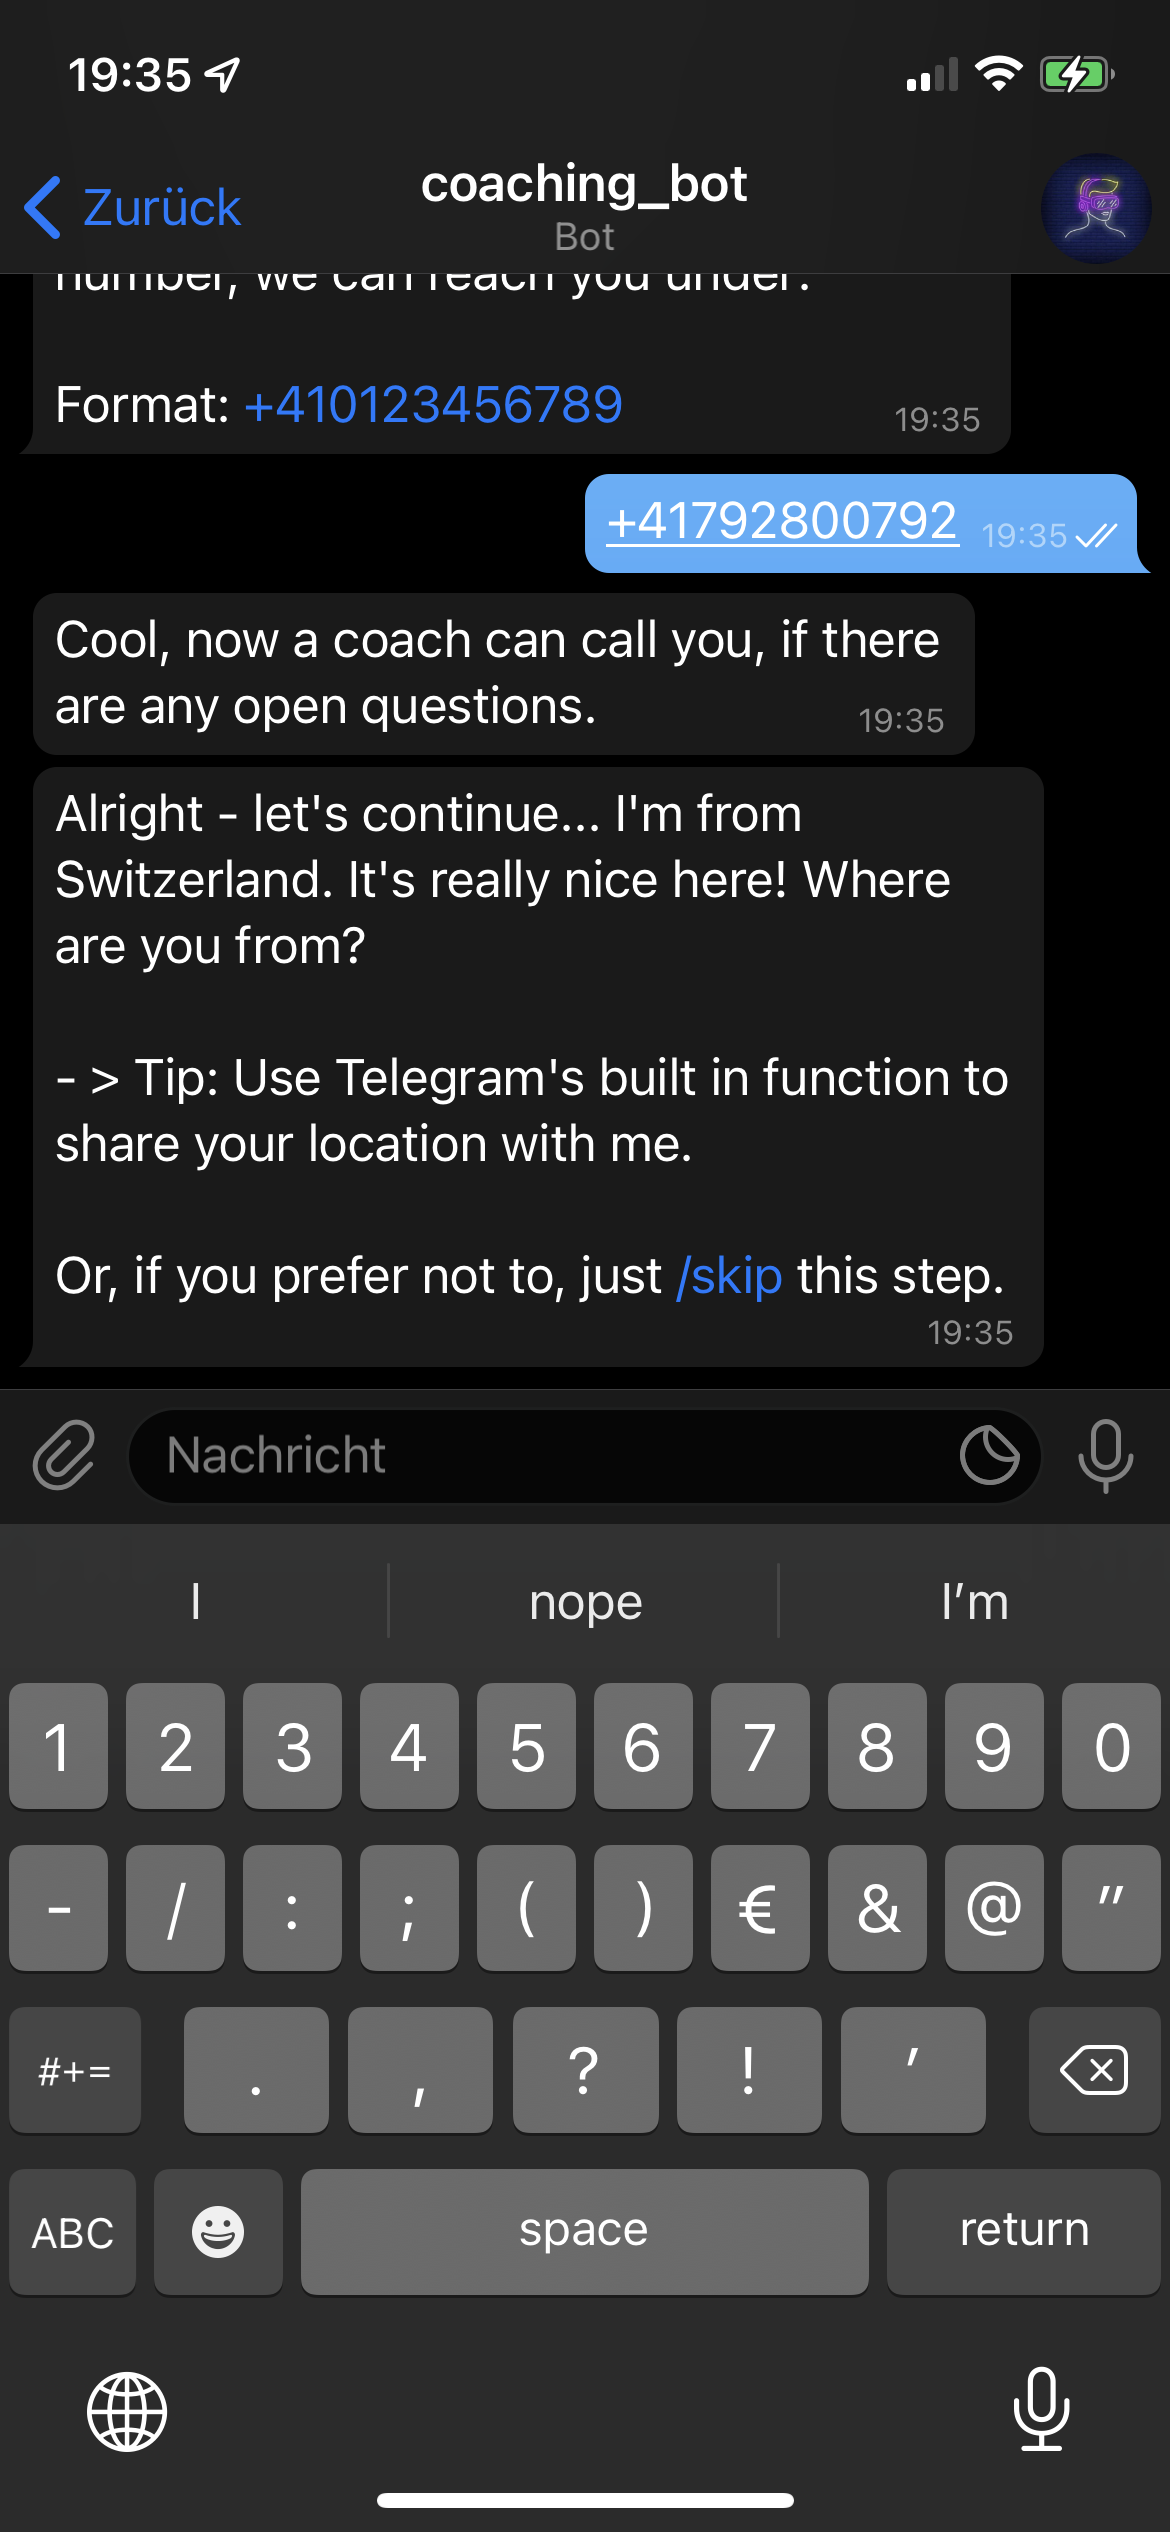
\includegraphics[width=\linewidth,height=300pt,keepaspectratio]{images/Screenshots/location.PNG}}
		
			\caption{Abfrage Telefonnummer und Standort}
		\end{minipage}
	\end{figure}


	% PAGE 03
	\begin{figure}
		\centering
		\begin{minipage}{.48\linewidth}
			\centering
			\subcaptionbox{Übergang zum Upload eines Fotos}
			{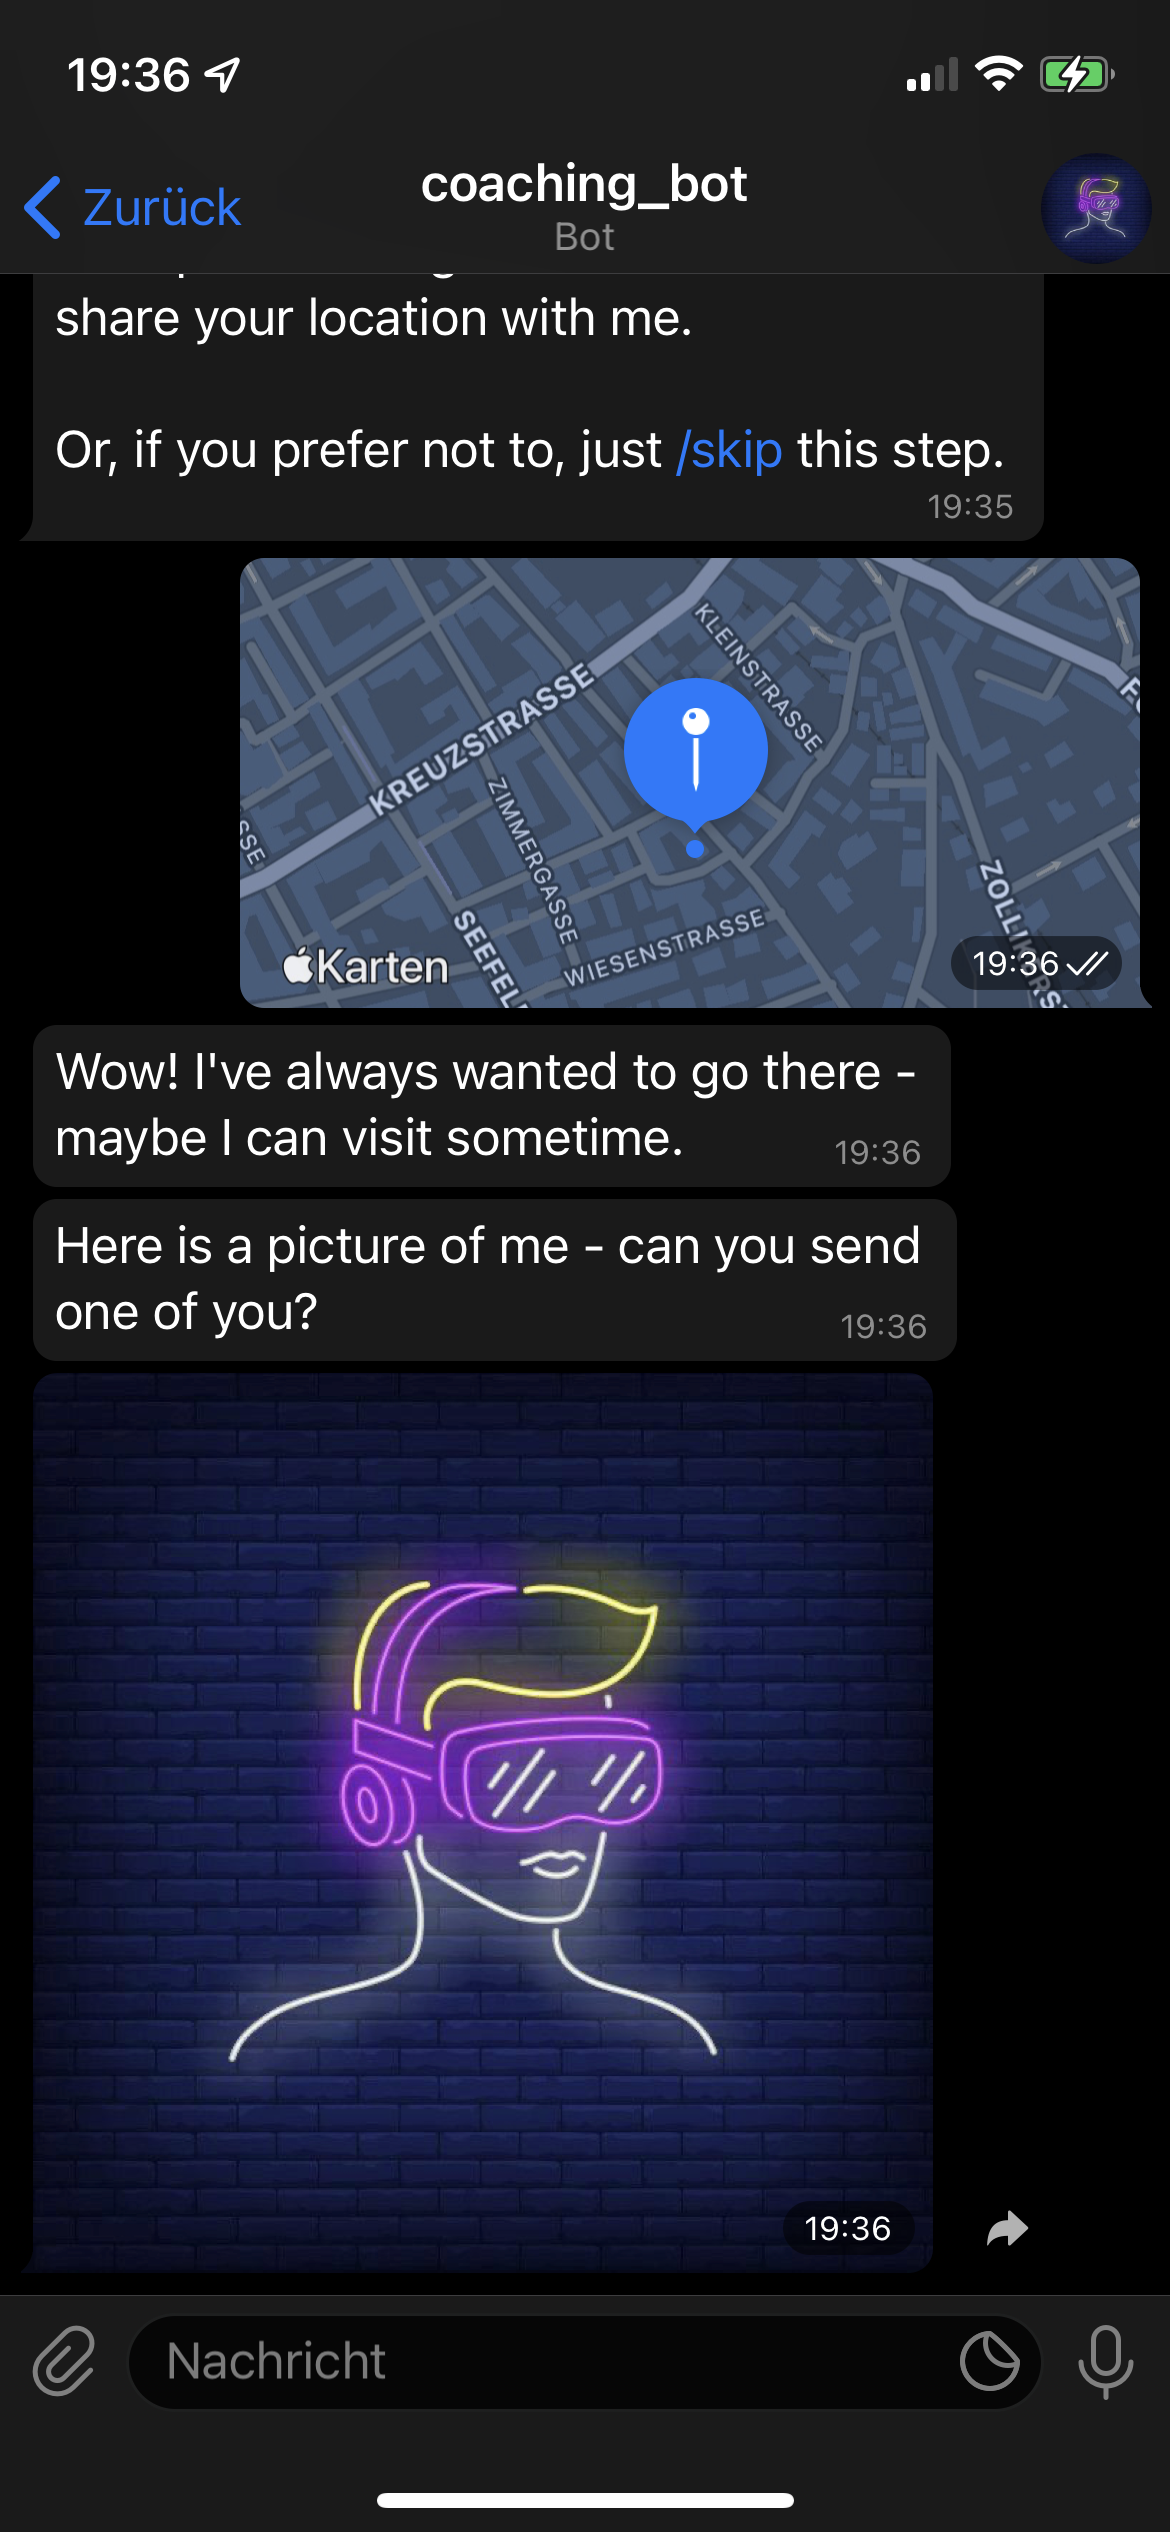
\includegraphics[width=\linewidth,height=300pt,keepaspectratio]{images/Screenshots/photo.PNG}}
		
			\subcaptionbox{Ende der Anmeldung und Übergang zur Terminauswahl}
			{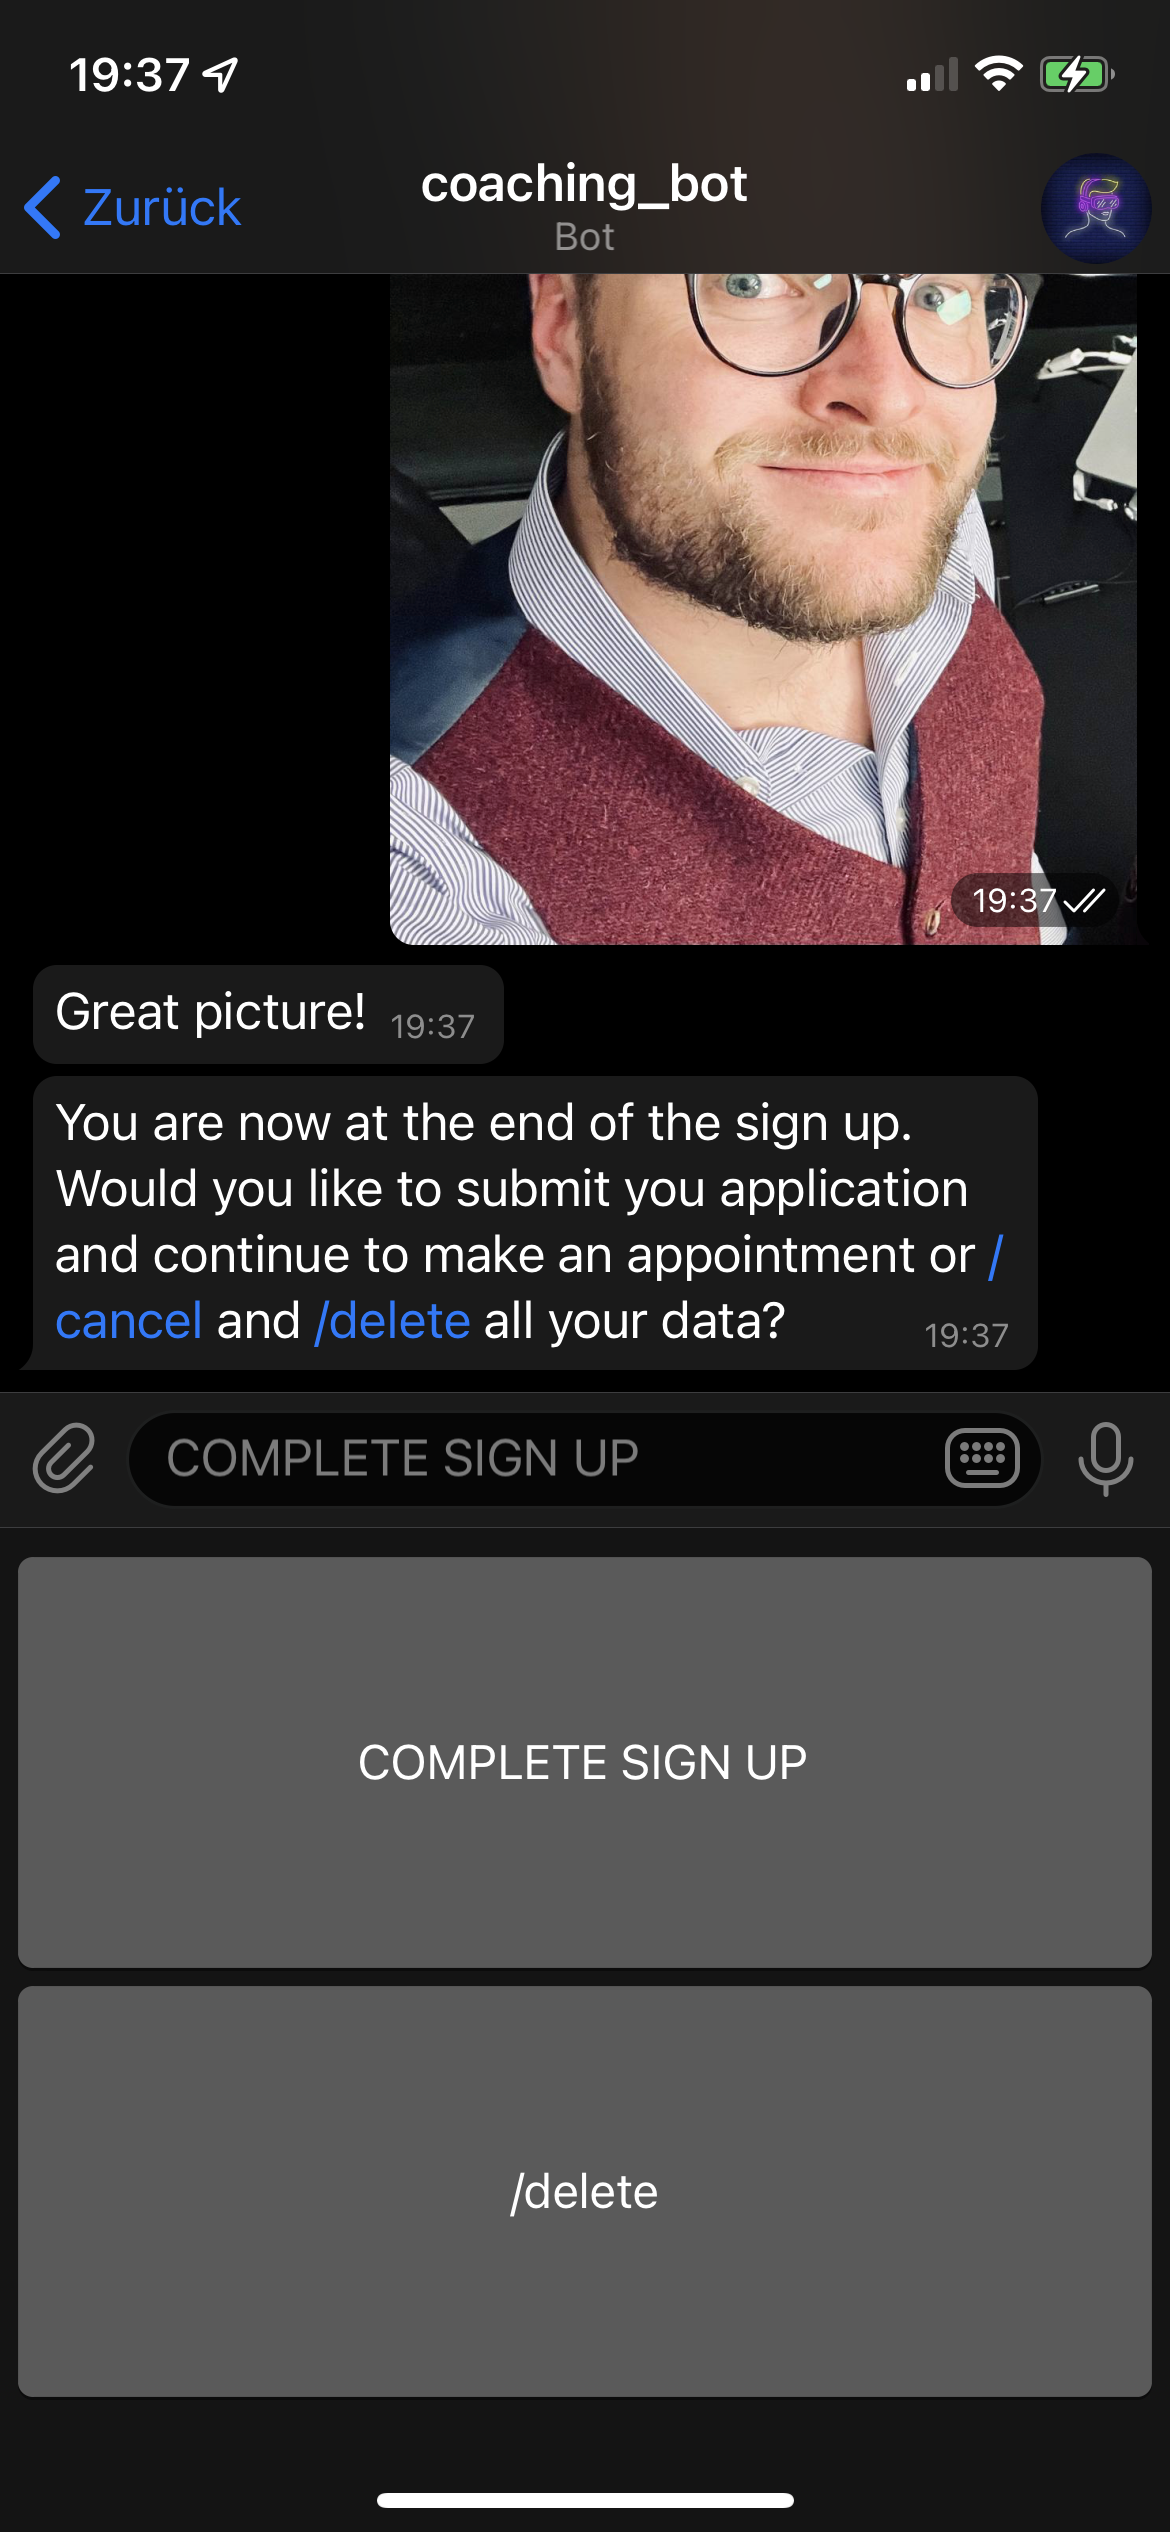
\includegraphics[width=\linewidth,height=300pt,keepaspectratio]{images/Screenshots/complete-sign-up.PNG}}
		
			\caption{Frage nach einem Bild des Nutzers und Abschluss des Sign-Ups}
		\end{minipage}\quad
		\begin{minipage}{.48\linewidth}
			\centering
			\subcaptionbox{Terminfindung}
			{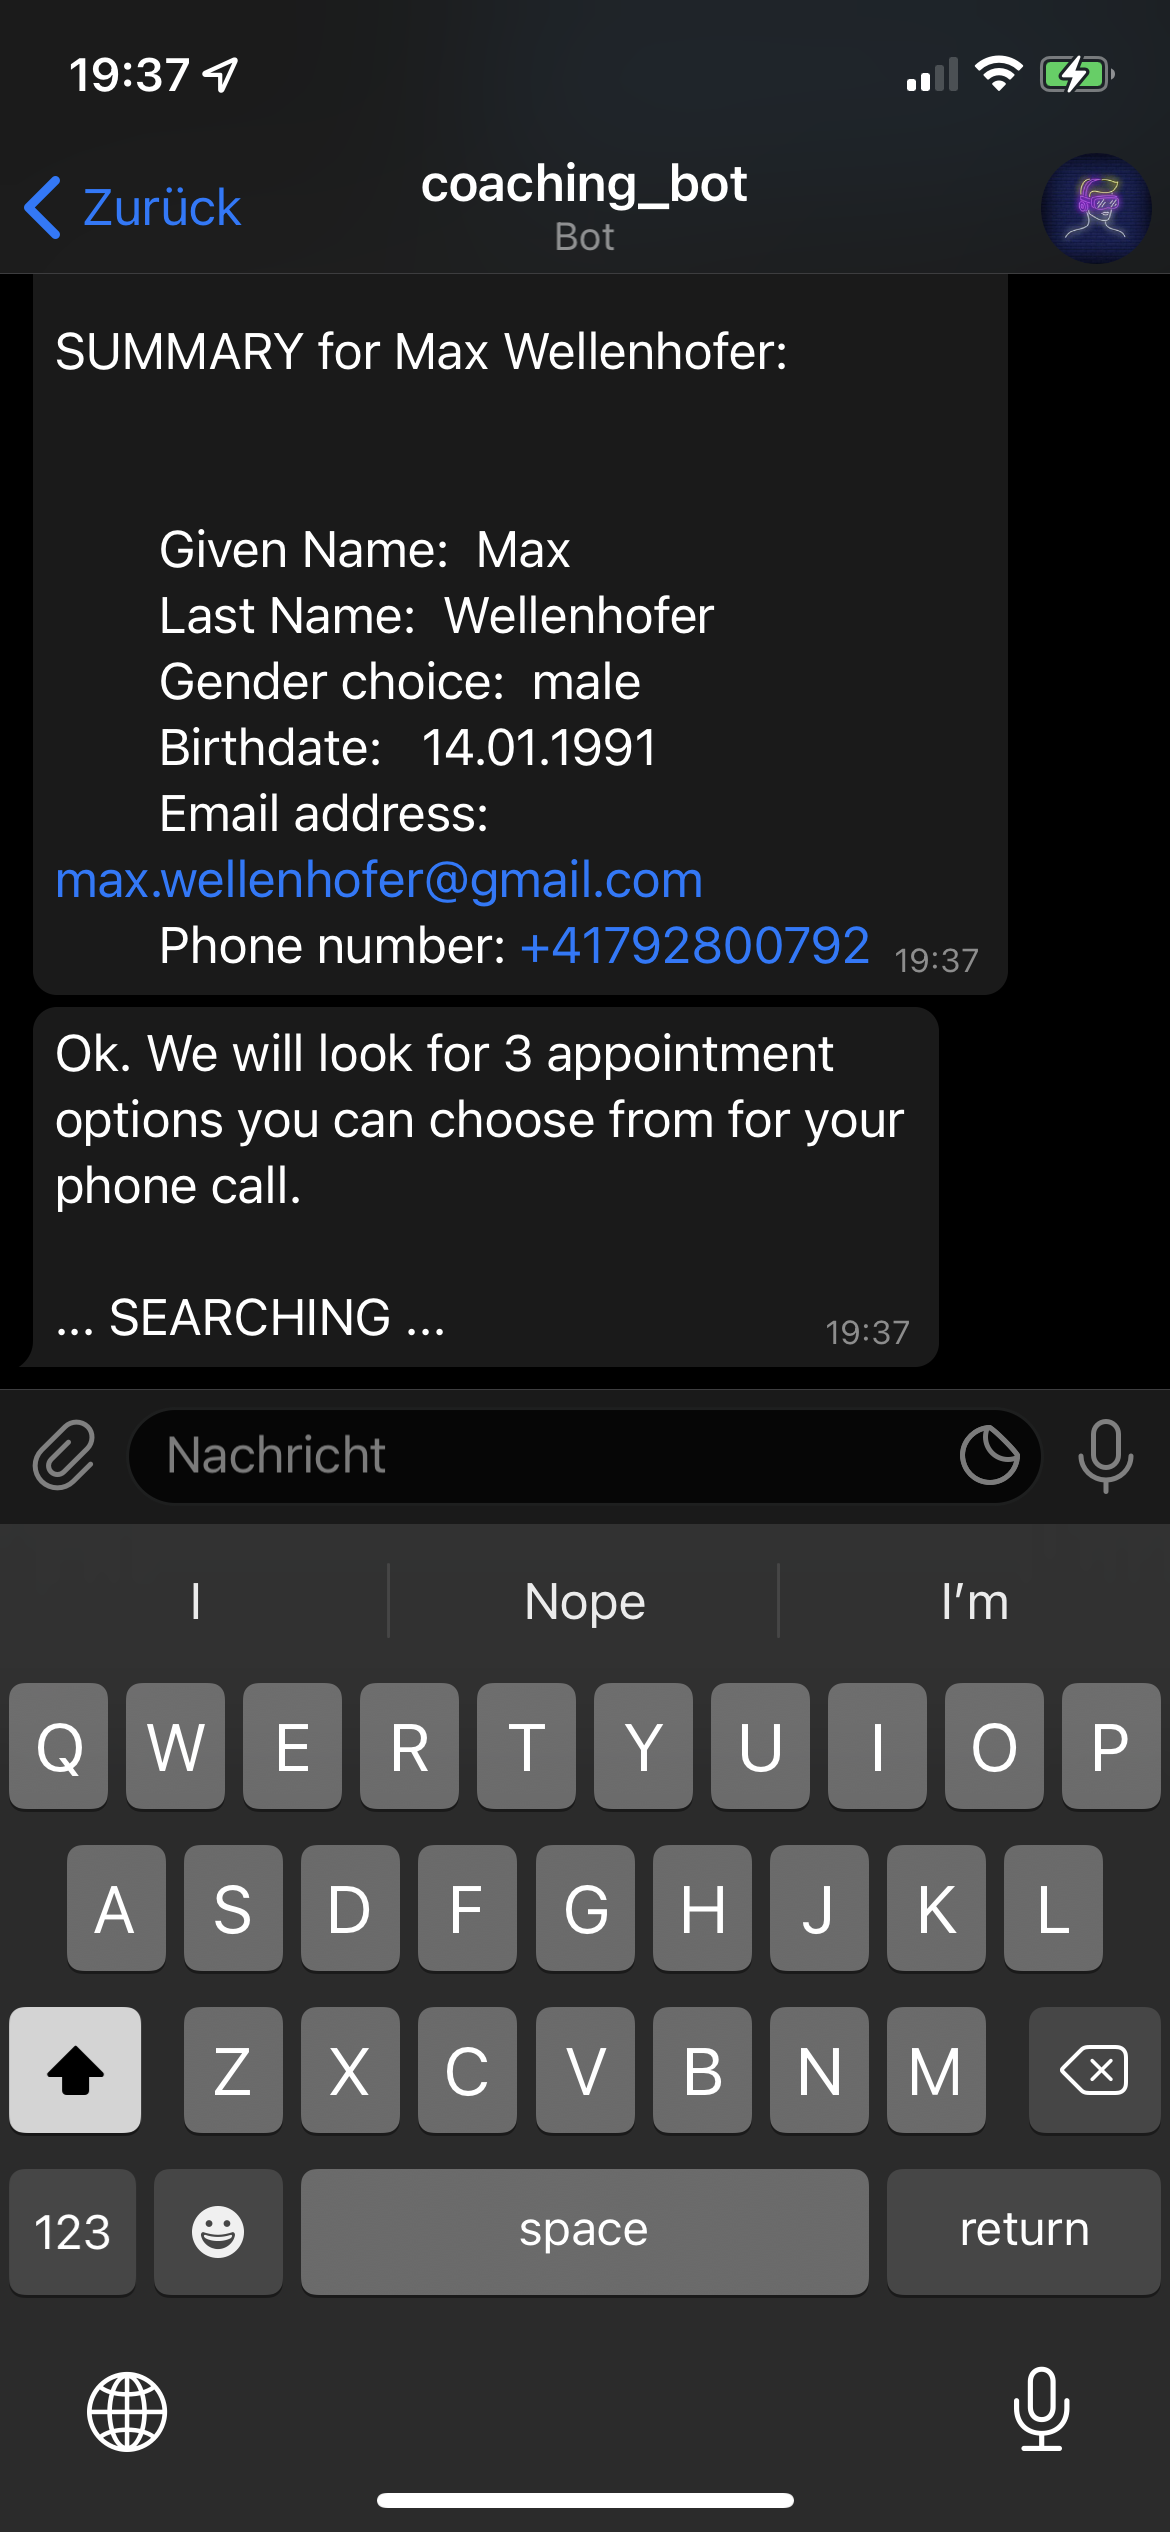
\includegraphics[width=\linewidth,height=300pt,keepaspectratio]{images/Screenshots/slot-search.PNG}}
		
			\subcaptionbox{Terminauswahl}
			{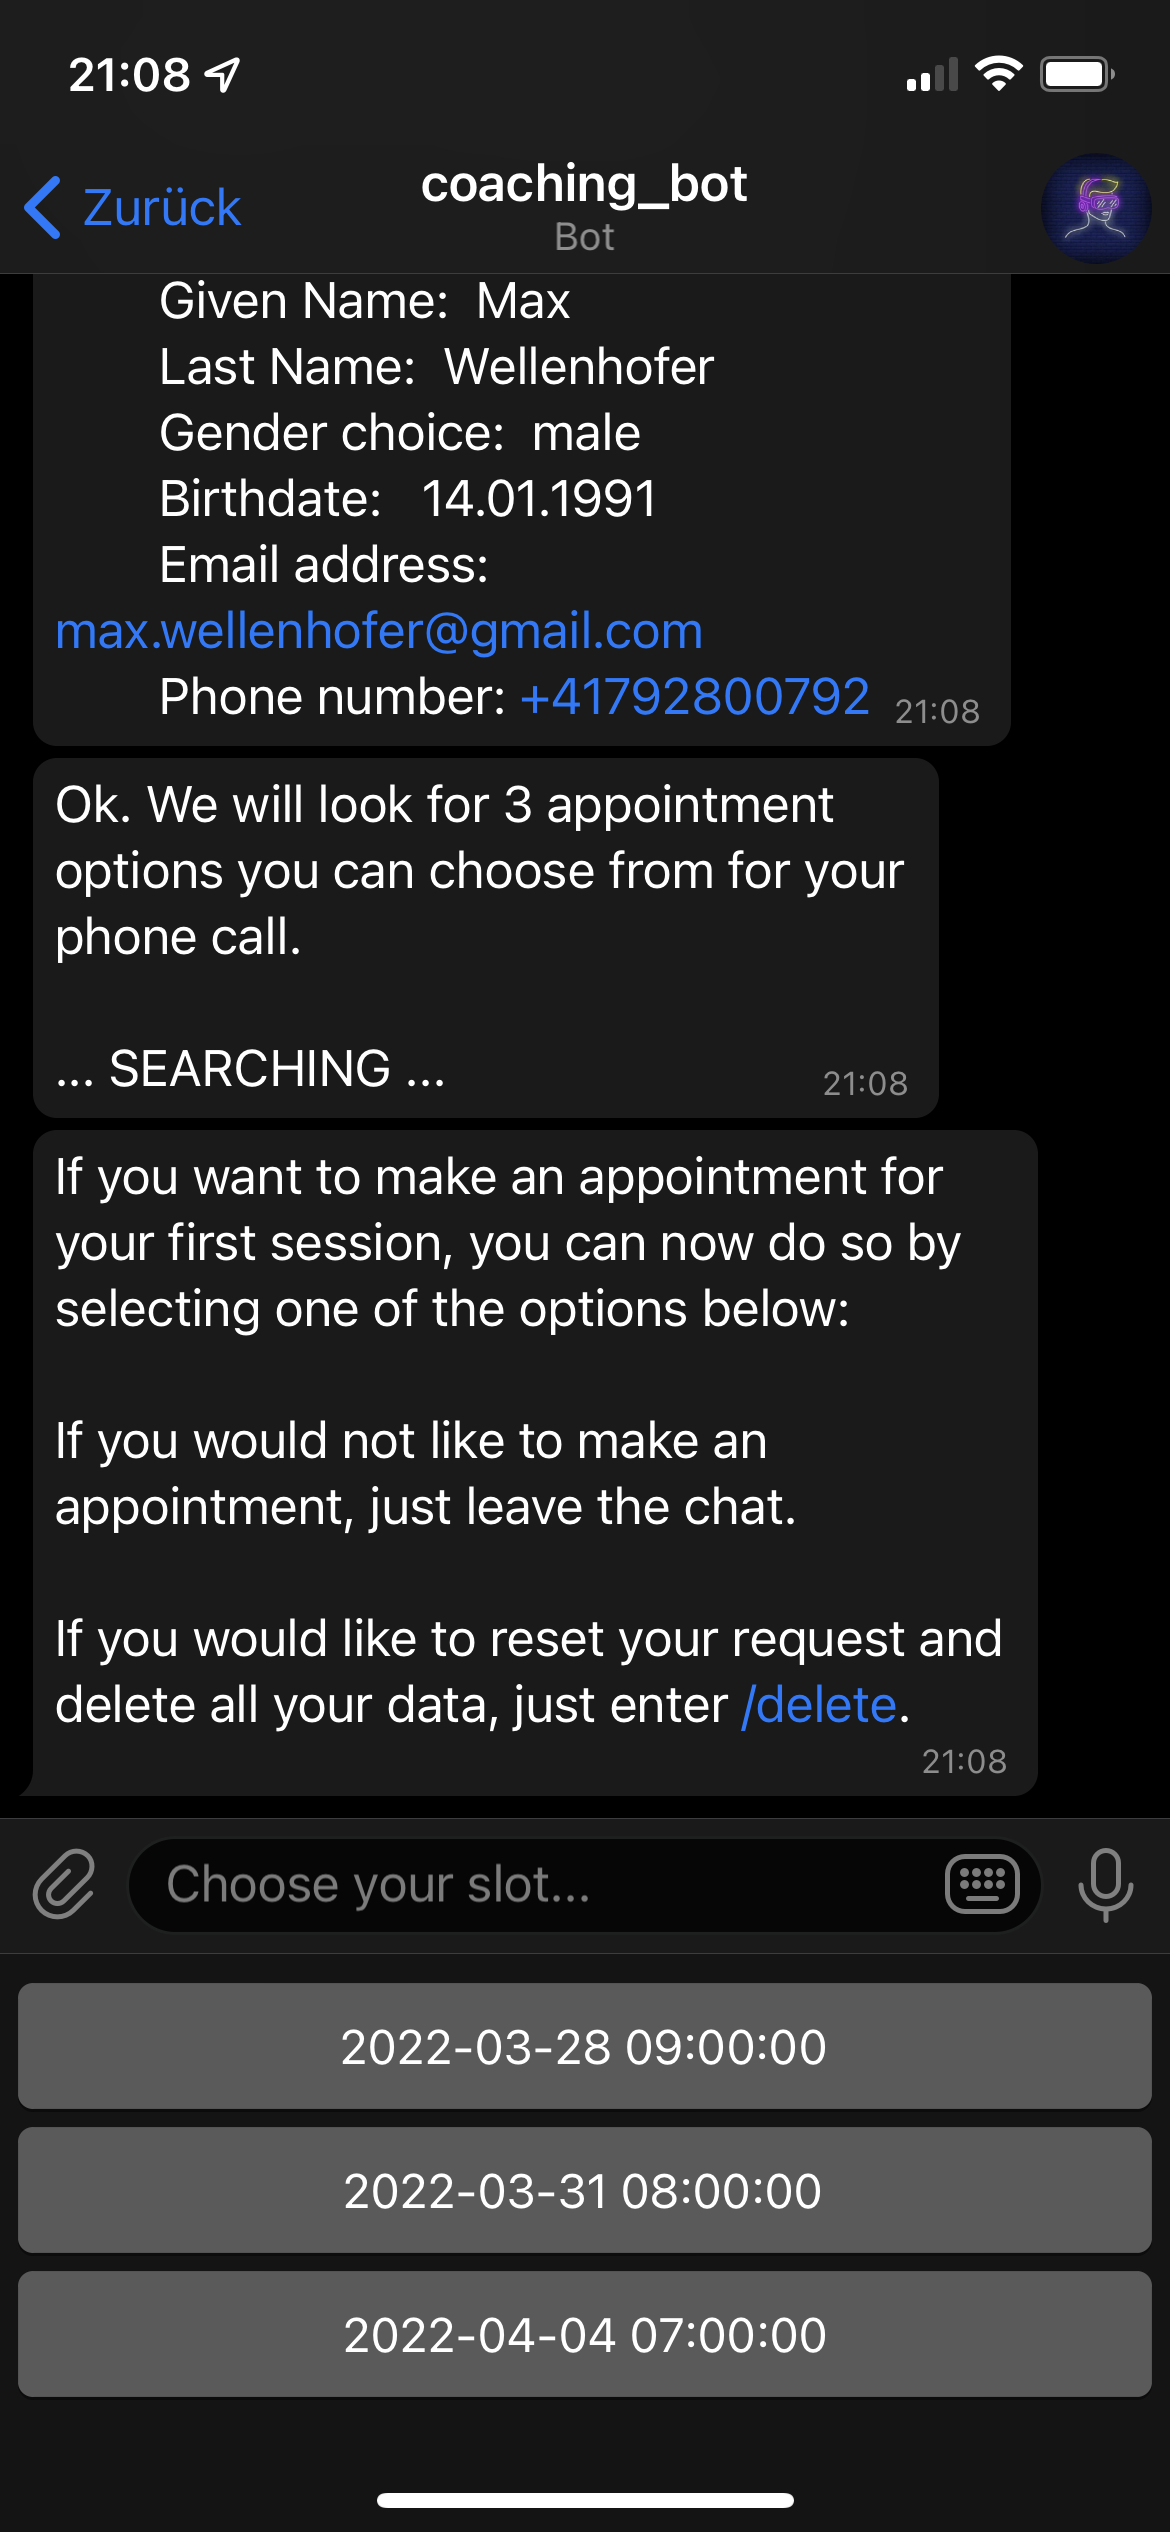
\includegraphics[width=\linewidth,height=300pt,keepaspectratio]{images/Screenshots/appointment-selection.PNG}}
		
			\caption{Terminsuche und -wahl}
		\end{minipage}
	\end{figure}


	% PAGE 04
	\begin{figure}
		\centering
		\begin{minipage}{.48\linewidth}
			\centering
			\subcaptionbox{Terminbestätigung}
			{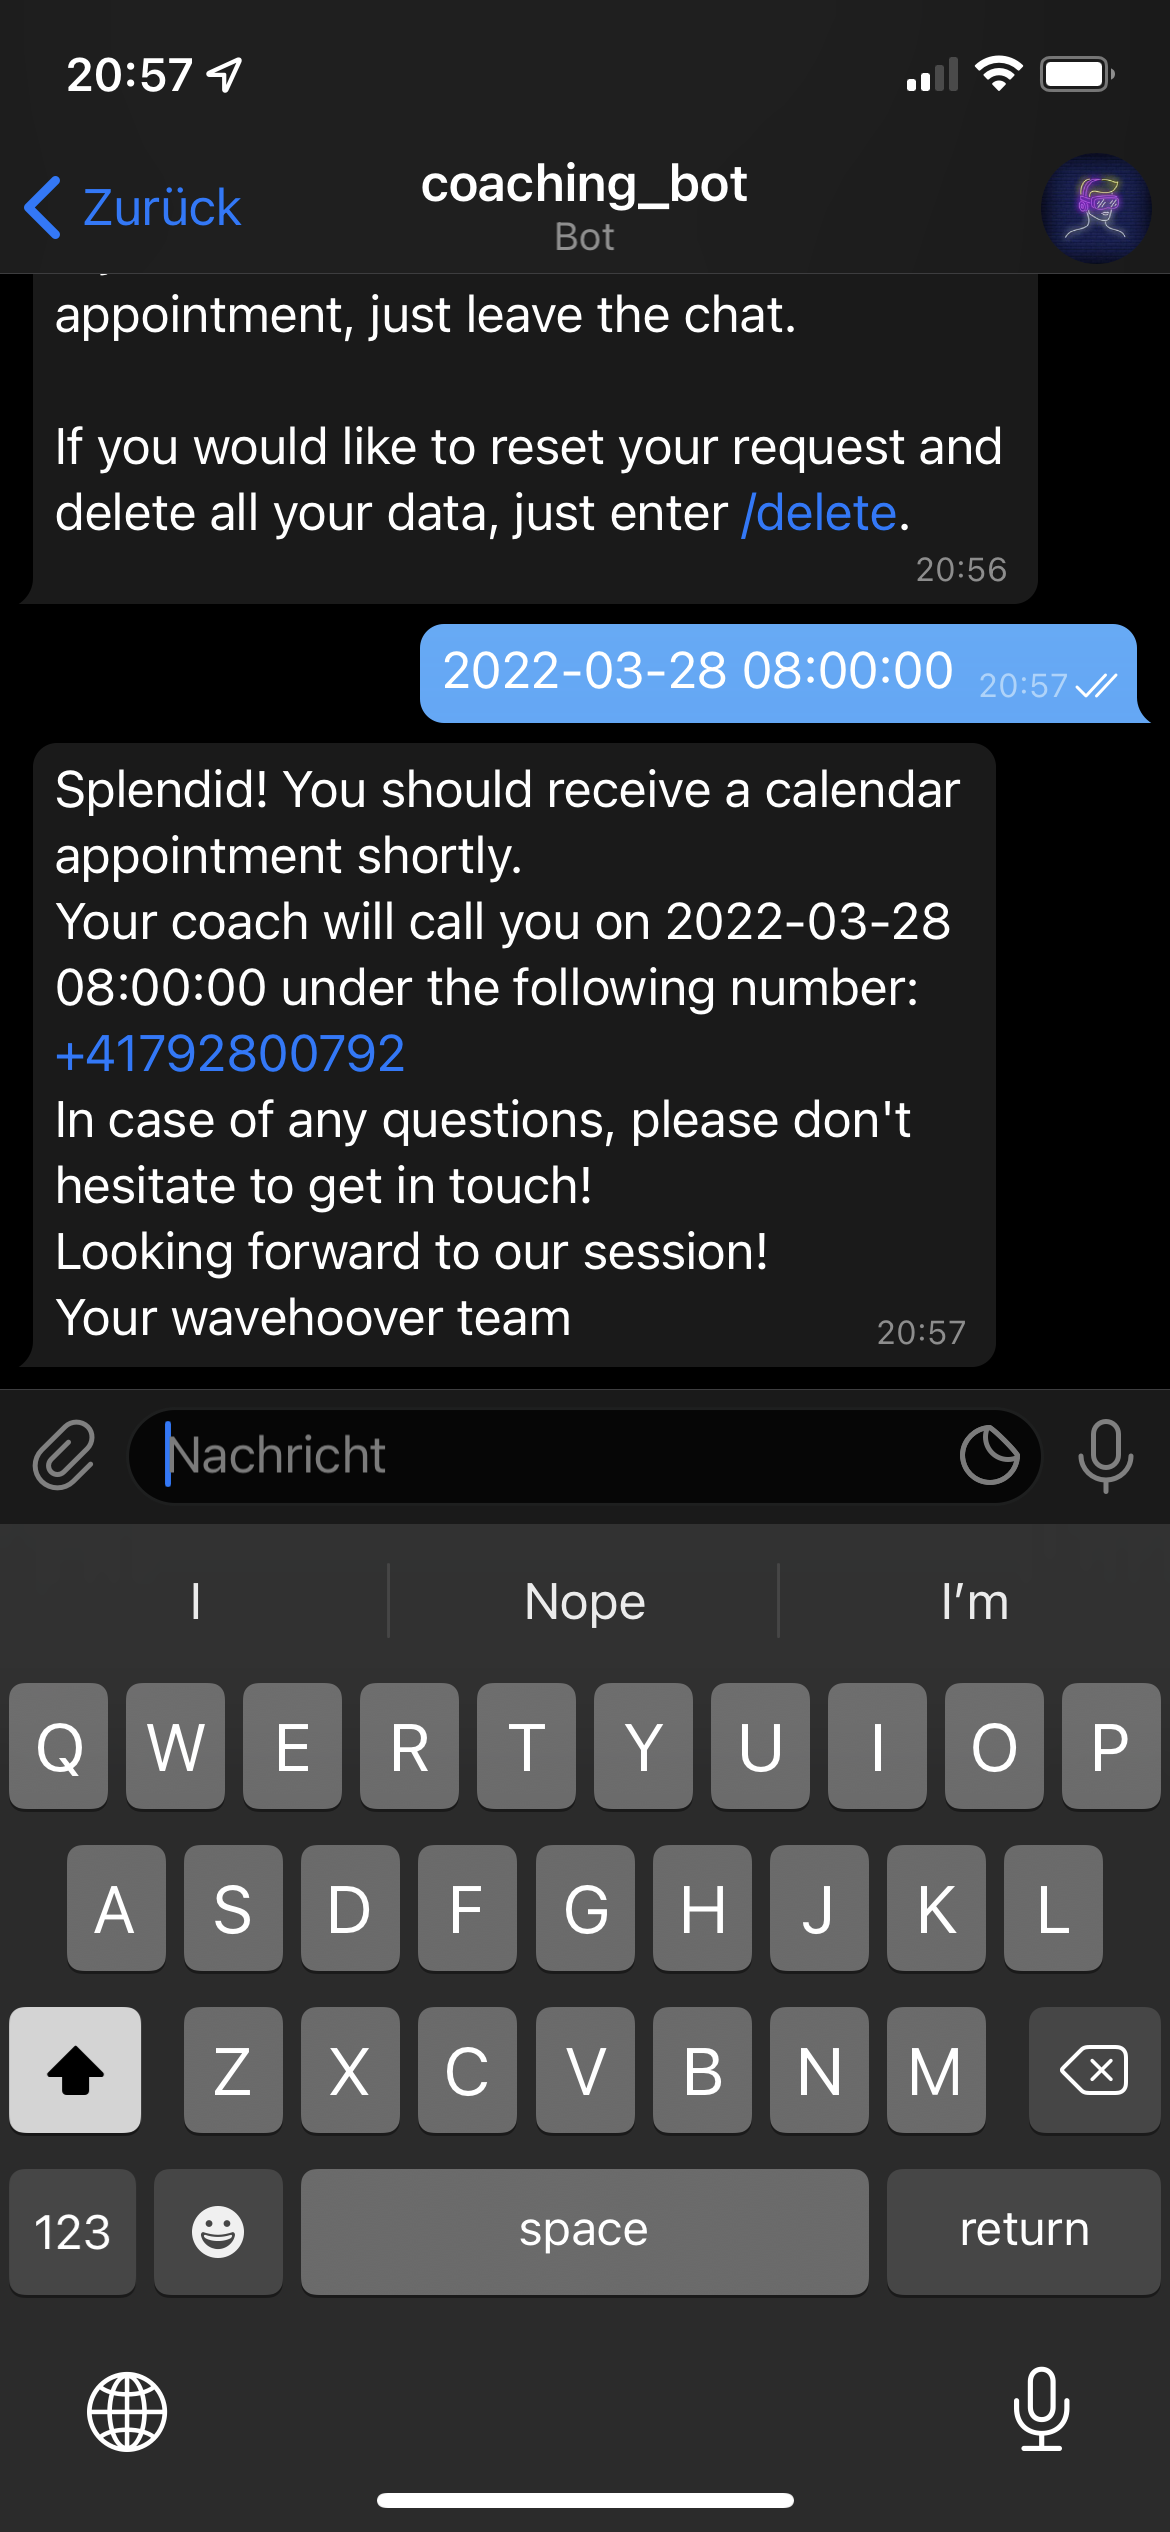
\includegraphics[width=\linewidth,height=300pt,keepaspectratio]{images/Screenshots/appointment-made.PNG}}
		
			\subcaptionbox{Kalendereinladung}
			{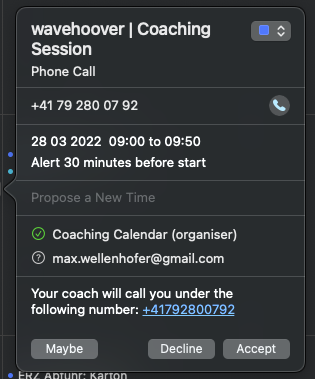
\includegraphics[width=\linewidth,height=300pt,keepaspectratio]{images/Screenshots/calendar-invite.png}}
		
			\caption{Bestätigung, dass Termin vereinbart wurde und die entsprechende Bestätigung per Kalender-Client}
		\end{minipage}\quad
		\begin{minipage}{.48\linewidth}
			\centering
			\subcaptionbox{Rückkehr zum Bot, wenn bereits ein Termin vereinbart wurde}
			{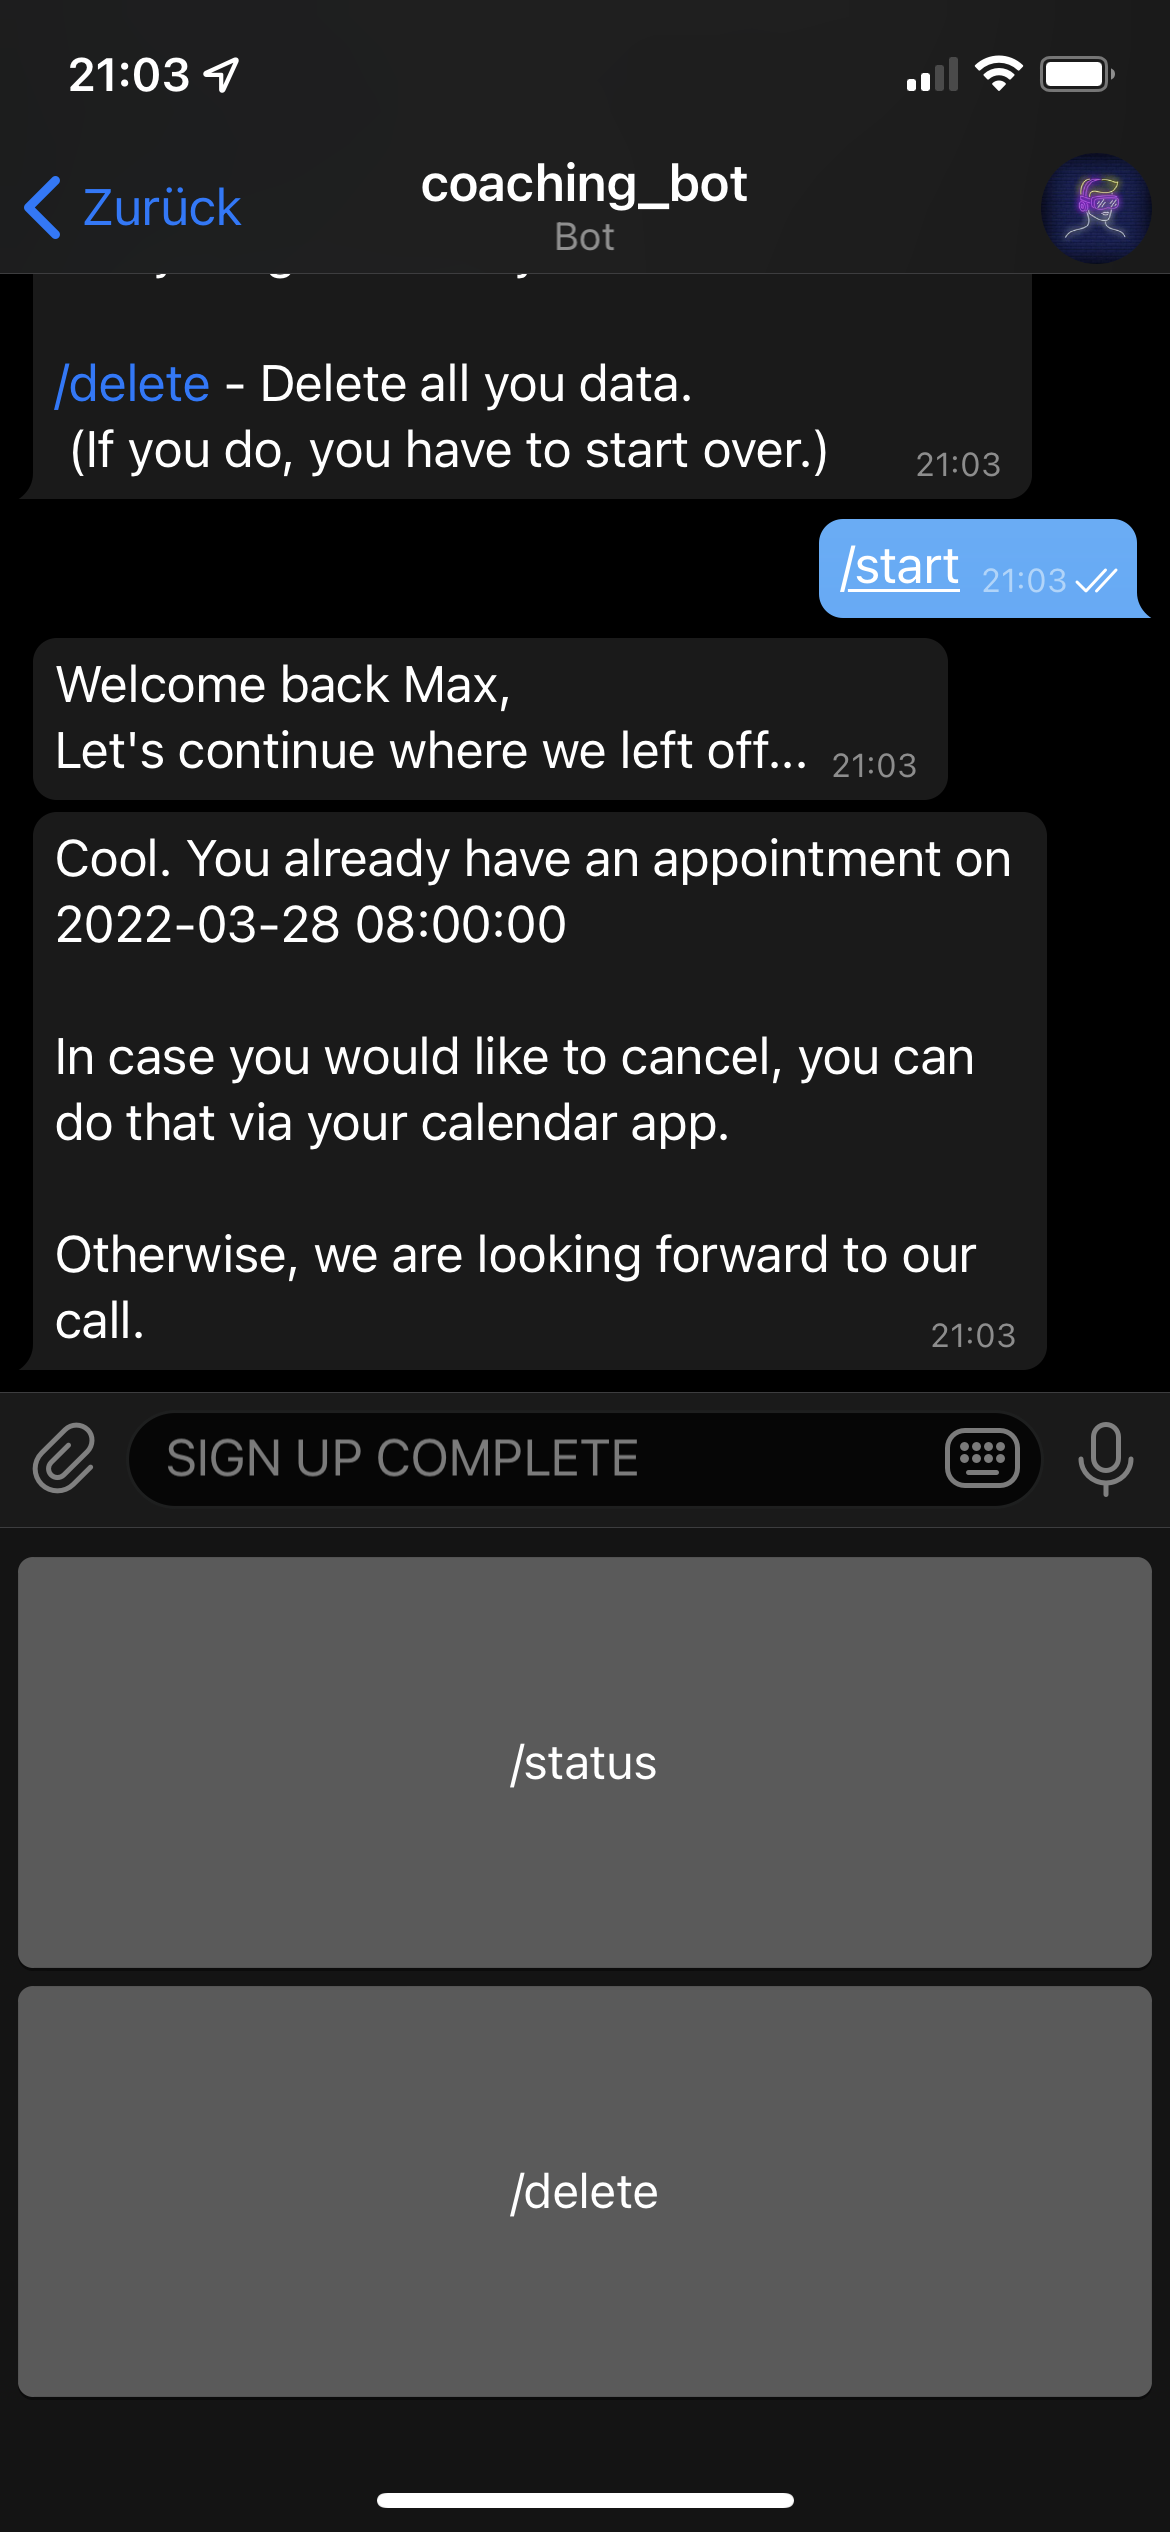
\includegraphics[width=\linewidth,height=300pt,keepaspectratio]{images/Screenshots/return-with-appointment.PNG}}
		
			\subcaptionbox{Statusabfrage und Hilfe}
			{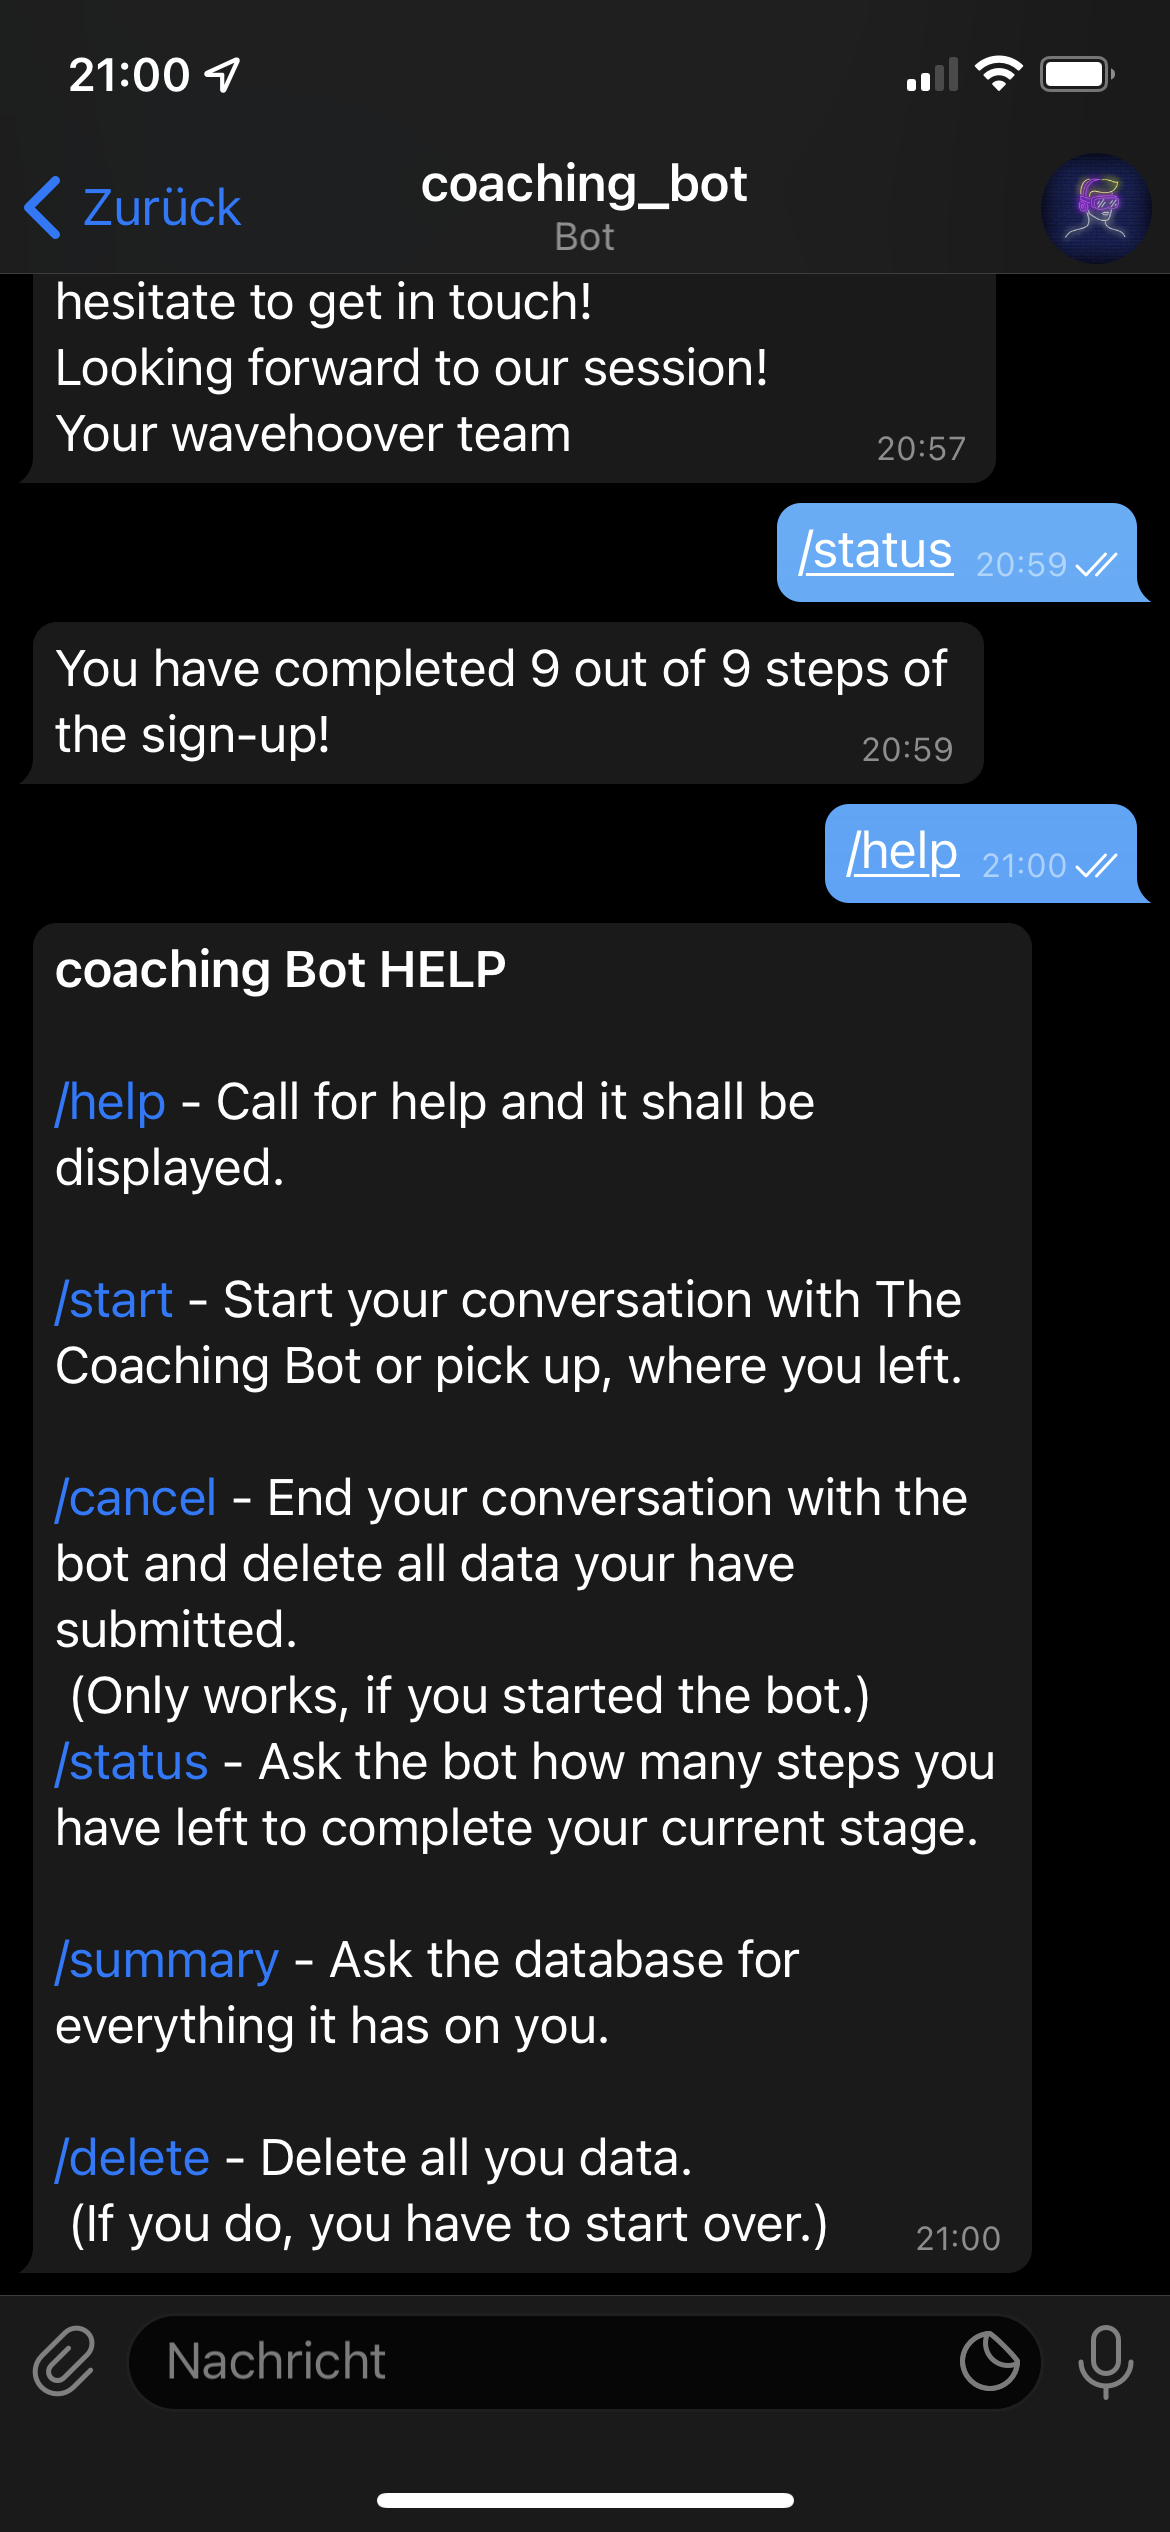
\includegraphics[width=\linewidth,height=300pt,keepaspectratio]{images/Screenshots/status-and-help.PNG}}
		
			\caption{Rückkehr des Nutzers nach Beendigung des Konversationsflusses und Ausgabe Meta-Funktionen}
		\end{minipage}
	\end{figure}


	% PAGE 05
	\begin{figure}
		\centering
		\begin{minipage}{.48\linewidth}
			\centering
			\subcaptionbox{Nutzerdaten löschen und Neustart des Bots}
			{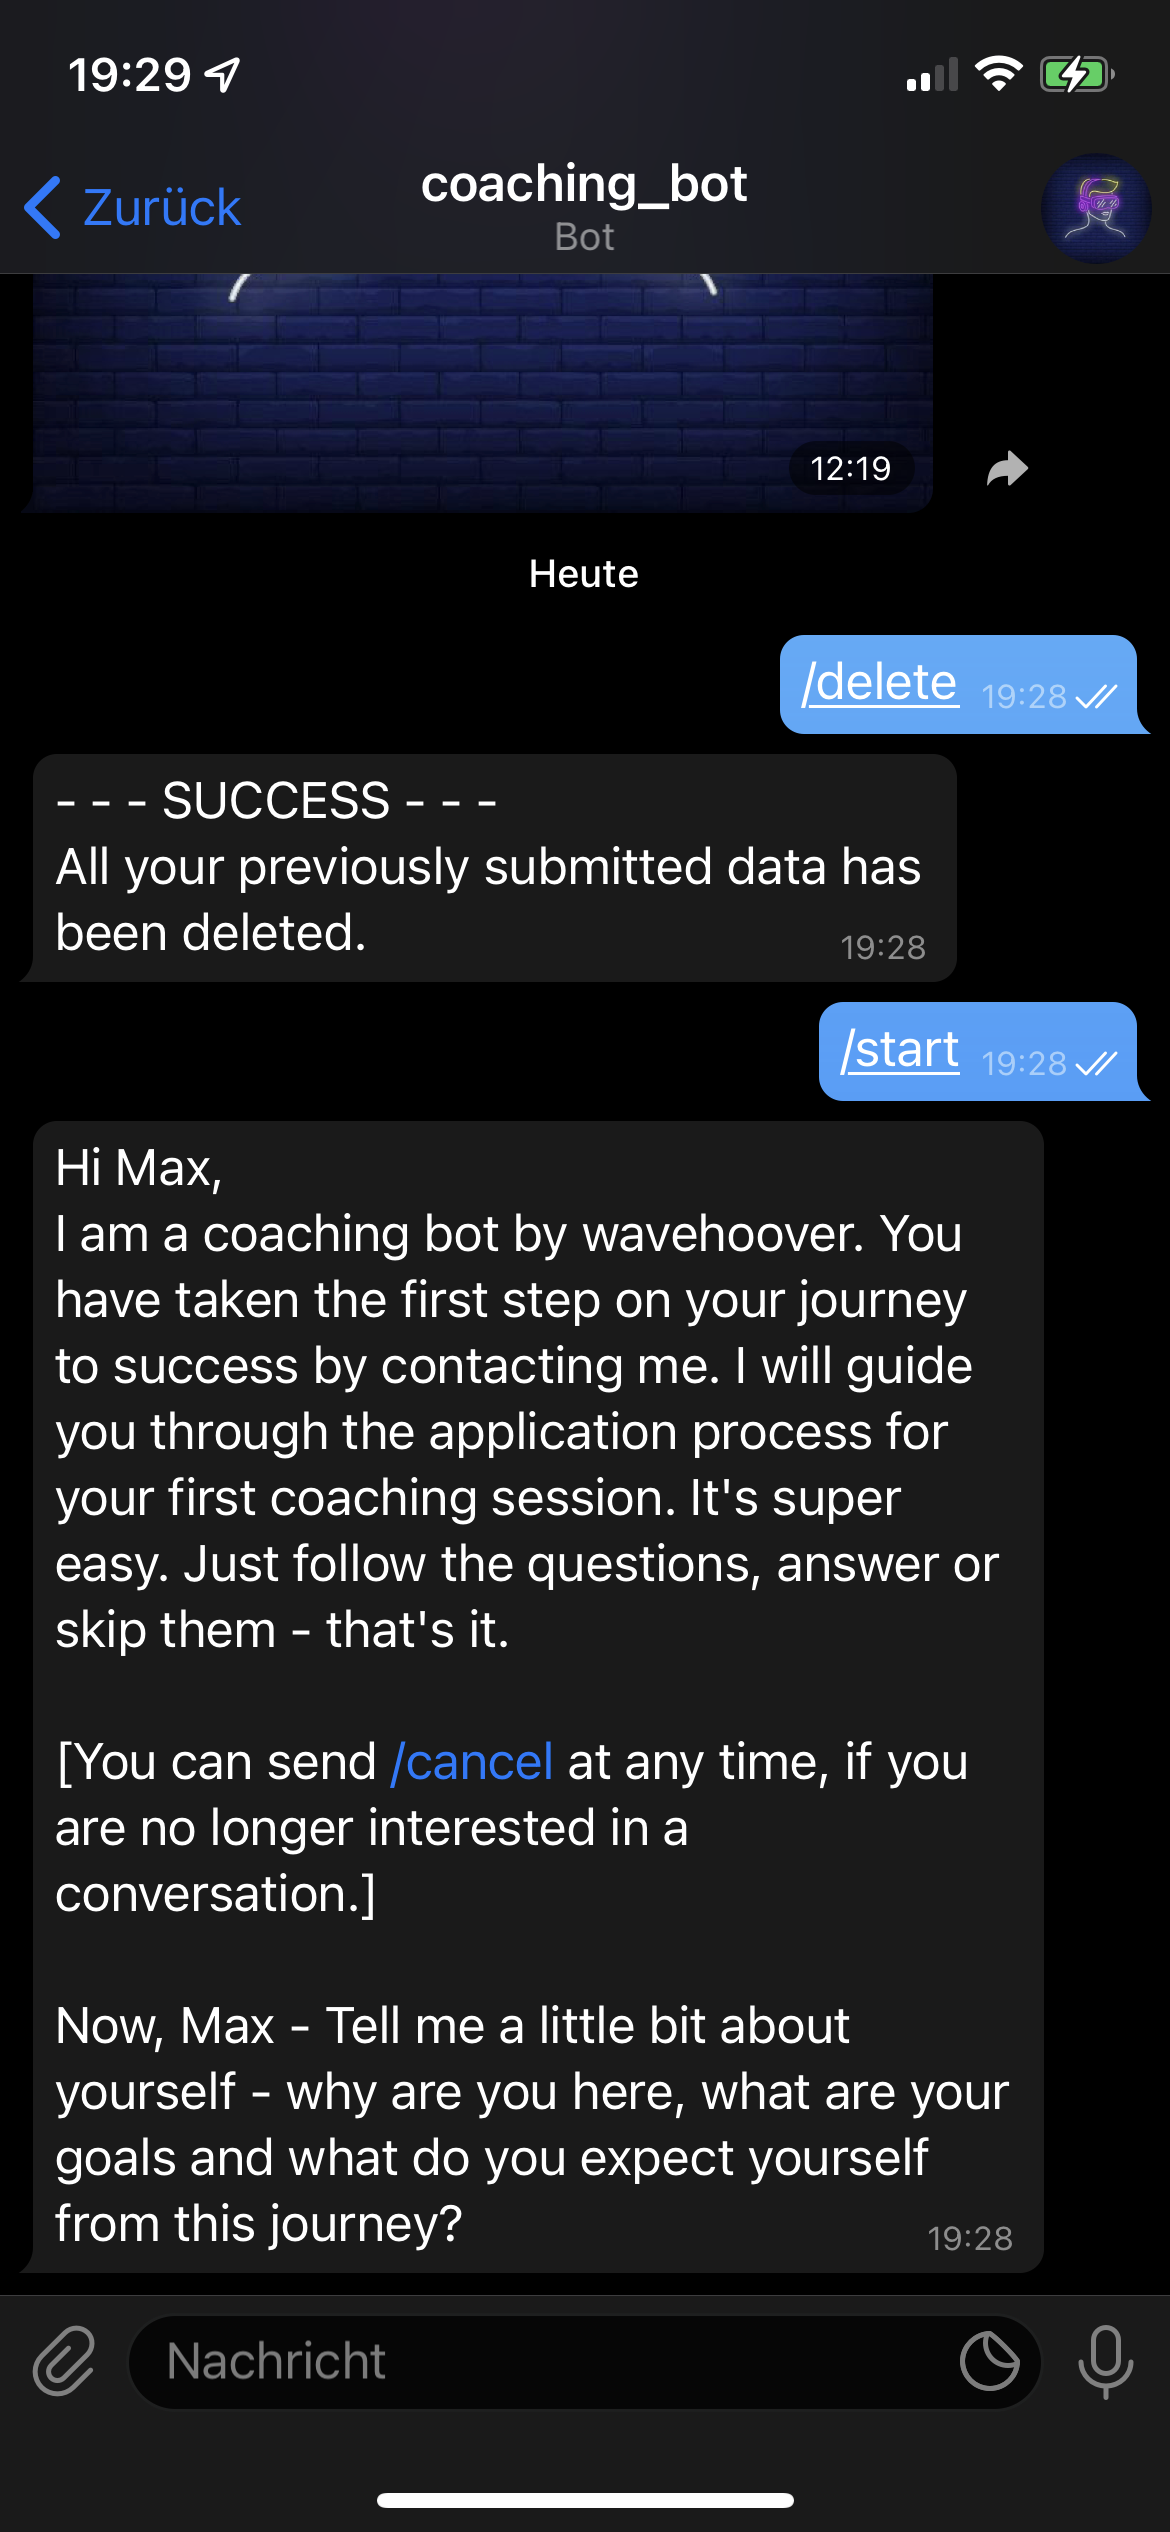
\includegraphics[width=\linewidth,height=300pt,keepaspectratio]{images/Screenshots/delete-and-restart.PNG}}
		
			\caption{Resultat aus \/delte und \/start}
		\end{minipage}\quad
	\end{figure}


	\begin{figure}
		\centering
		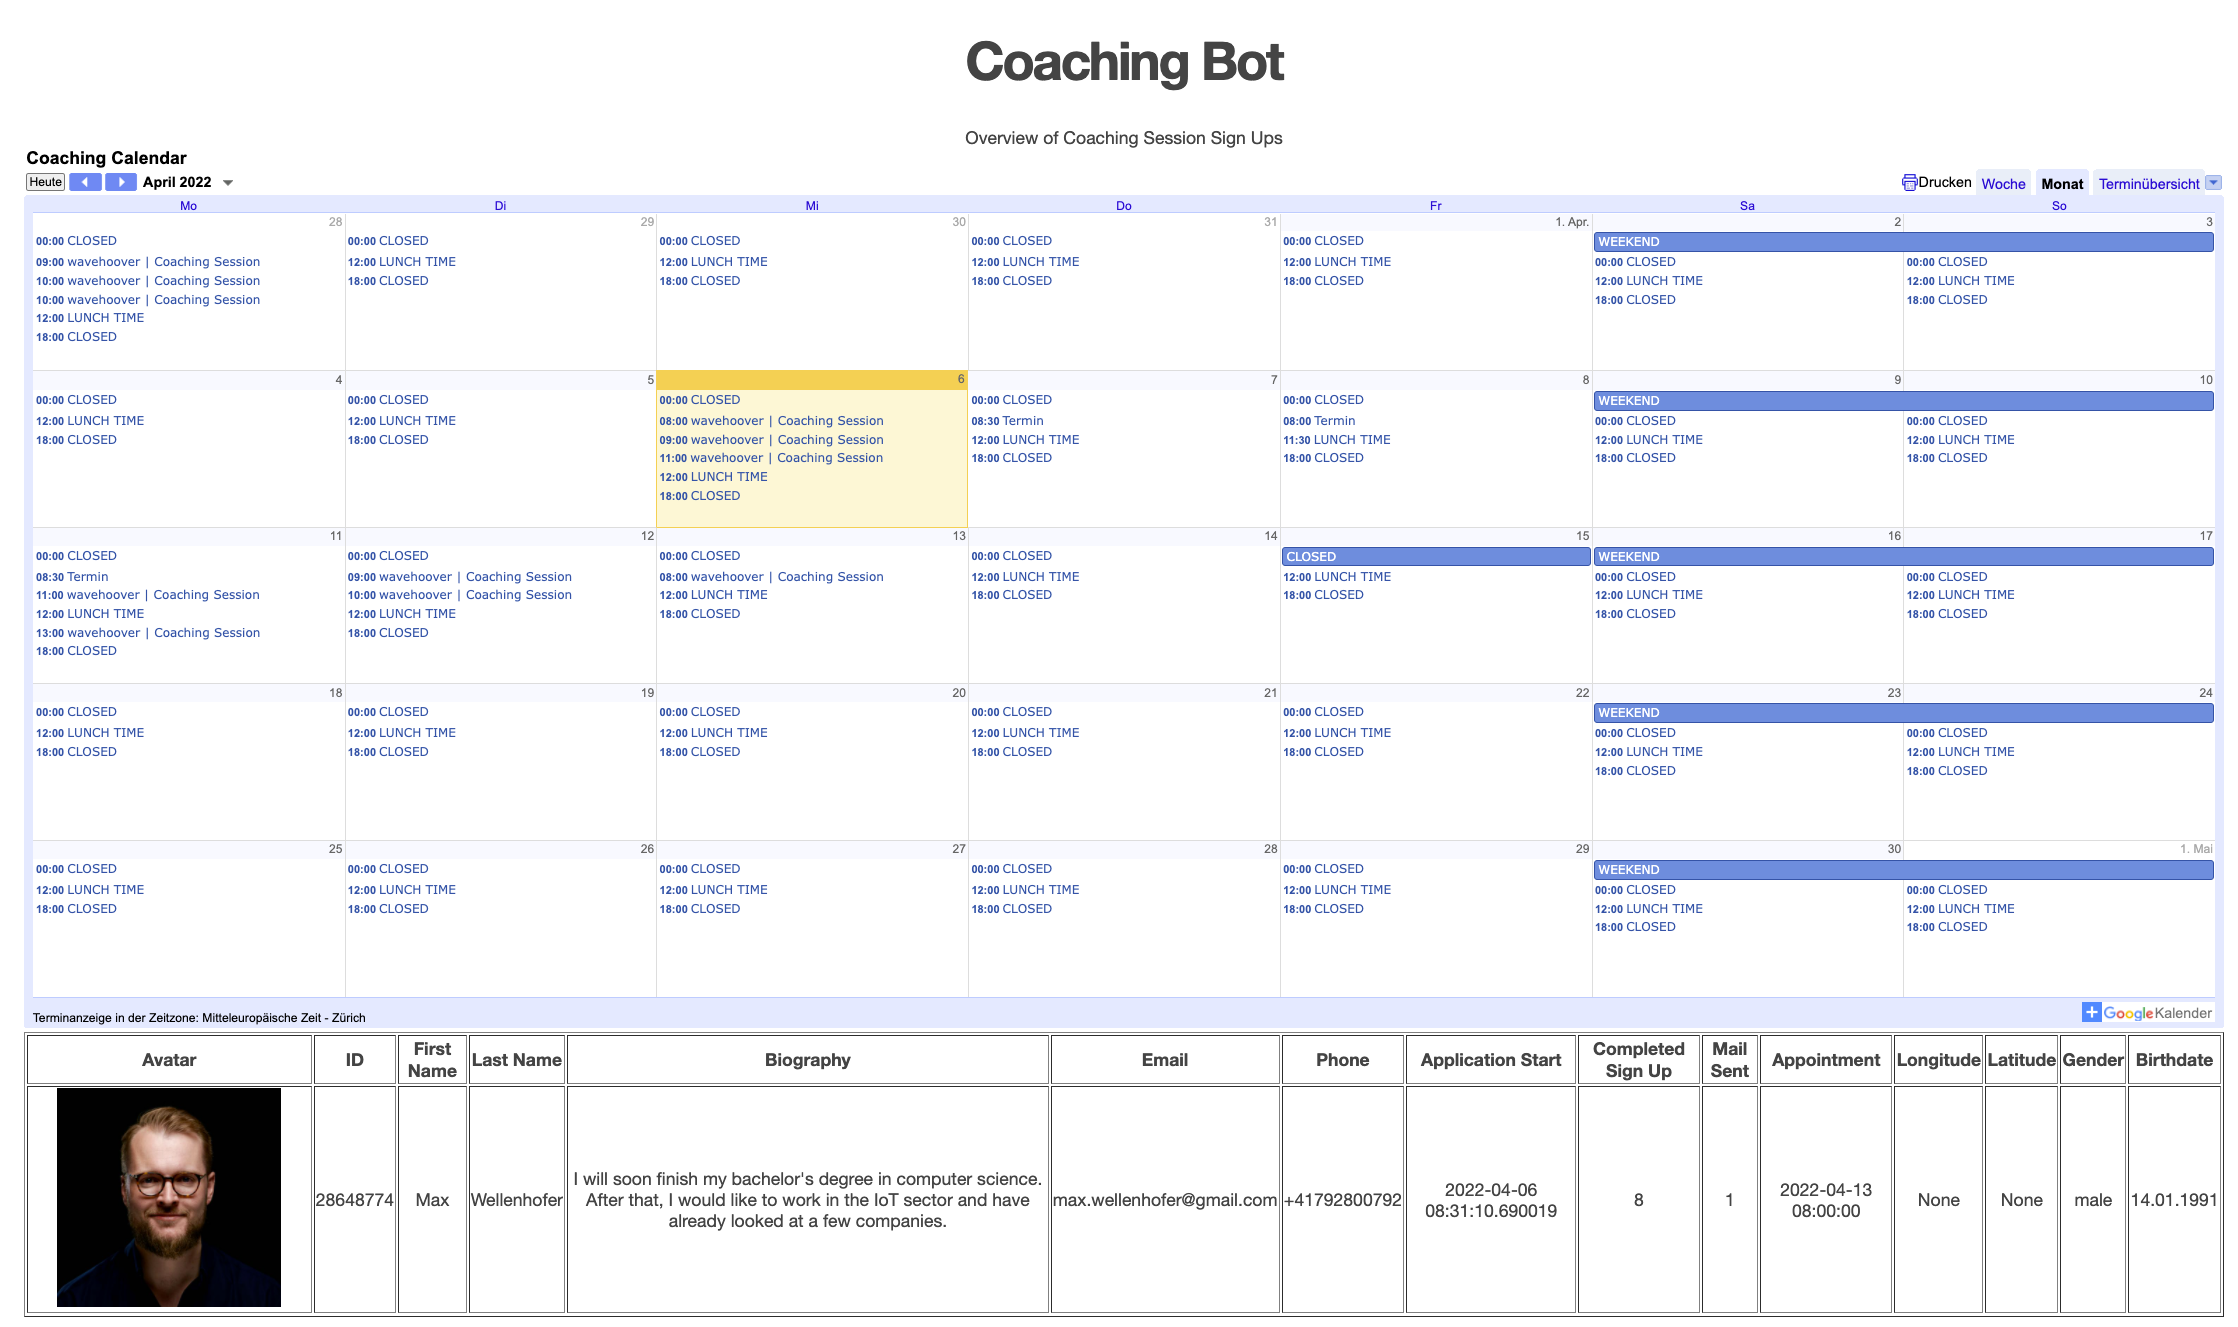
\includegraphics[width=1\textwidth]{images/Screenshots/web-gui.png}
		\caption{Coach-Übersicht mit Kalender und Nutzer-Informationen im Listenformat}
		\label{fig: scs..web-gui}
	\end{figure}

